\subsection{Extracción de los procesos con DISCO}

Del dataset proporcionado se extraerán los campos de información más importantes:
\begin{enumerate}
\item El identificador del caso, extraído de una clave aleatoria generada al principio de cada operación \texttt{LOGIN} y que distingue de manera unívoca cada sesión de trabajo de los estudiantes.
\item El agente, que se refiere al nombre del grupo de estudiantes.
\item La fecha y hora a la que se registró la transacción.
\item El campo actividad (\texttt{Activity}), que refleja la acción de los alumnos en el mundo virtual.
\item Varios campos de tipo recurso (\texttt{Resource}) que proporcionan información adicional que puede sernos de utilidad a la hora de filtrar los registros.
\end{enumerate}

Se importarán el dataset de dos maneras diferentes, con el objetivo de estudiar tanto la frecuencia con que cada problema o mapa ha sido visitado como las acciones compuestas mapa-porcentaje superado. En la primera importación la \texttt{Activity} es la columna \emph{Objeto} mientras que en la segunda es la columna \emph{Compuesto} tal y como puede verse en las Figuras \ref{fig:DISCO1} y \ref{fig:DISCO2}.

\begin{figure}[H]
    \centering
    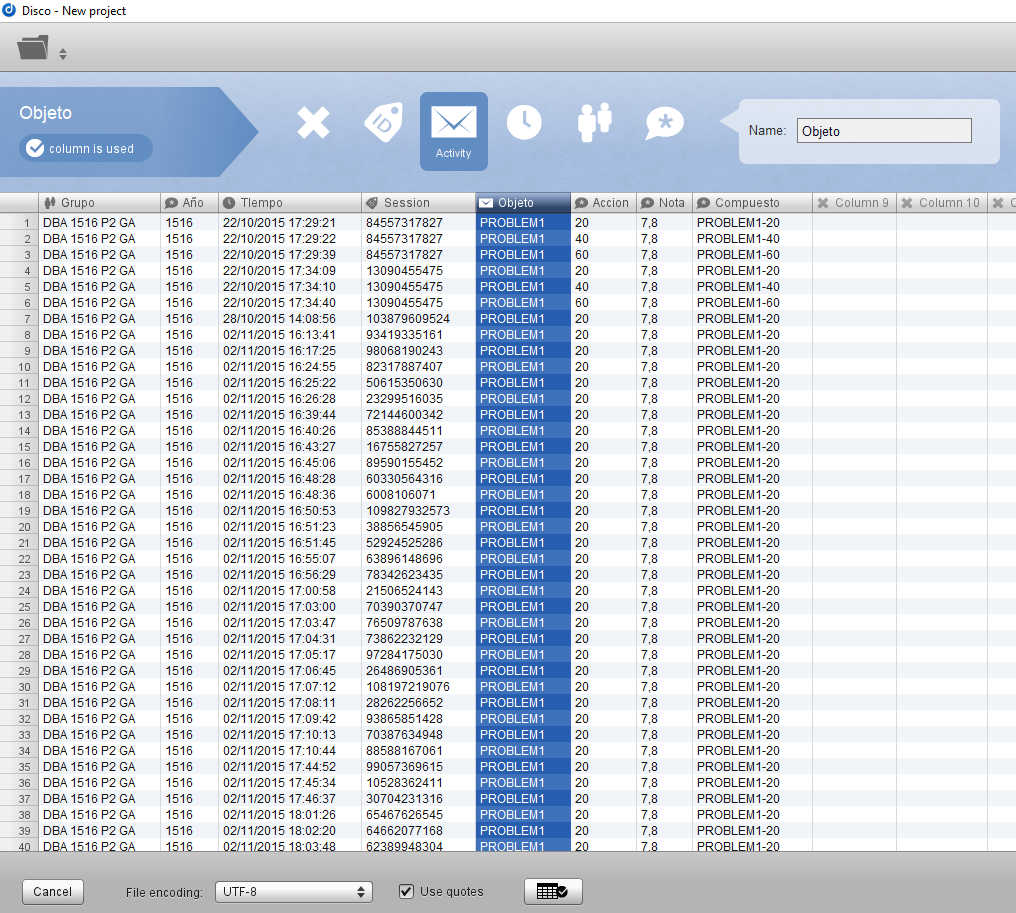
\includegraphics[width=0.90\textwidth]{imagenes/DISCO_map/DISCO_cut.png}
    \caption{Análisis de procesos del dataset compuesto (acción mapa).}
    \label{fig:DISCO1}
\end{figure}

\begin{figure}[H]
    \centering
    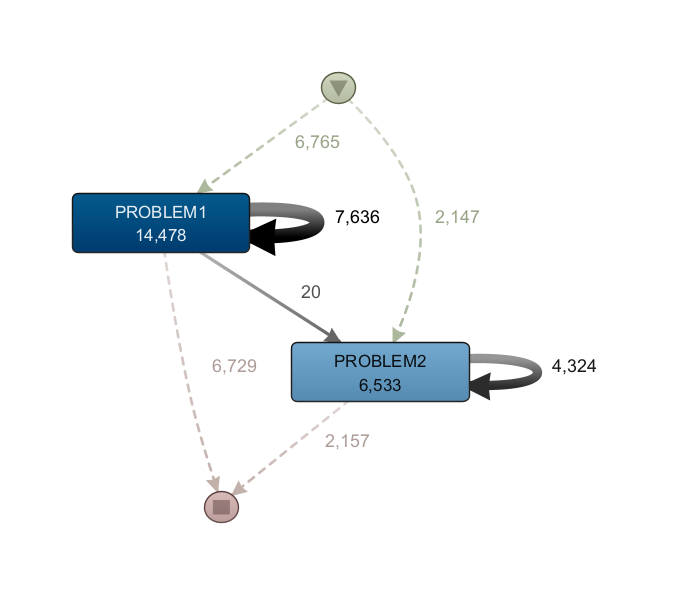
\includegraphics[width=0.75\textwidth]{imagenes/DISCO_map/Dataset Fusionado.png}
    \caption{Análisis de procesos del dataset compuesto (acción mapa).}
    \label{fig:datasetFusionado}
\end{figure}

\begin{figure}[H]
    \centering
    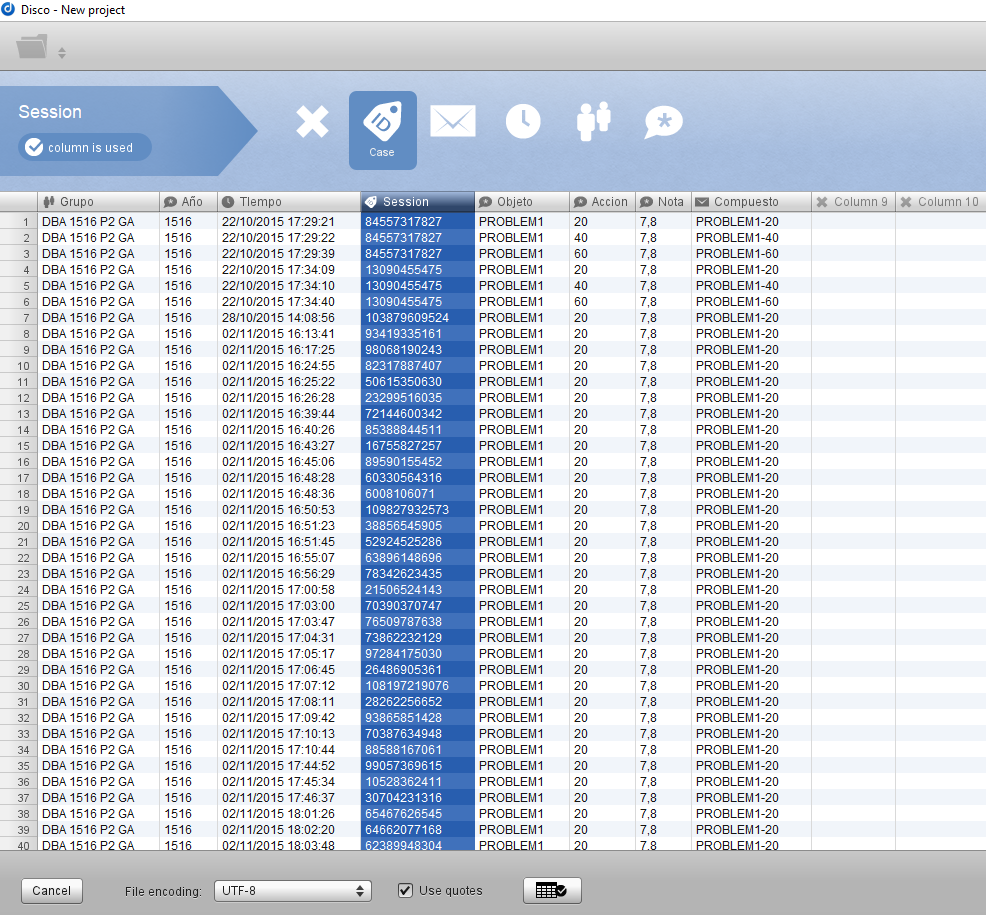
\includegraphics[width=0.90\textwidth]{imagenes/DISCO_compound/DISCO_cut.png}
    \caption{Análisis de procesos del dataset compuesto (acción compuesta).}
    \label{fig:DISCO2}
\end{figure}

\begin{figure}[H]
    \centering
    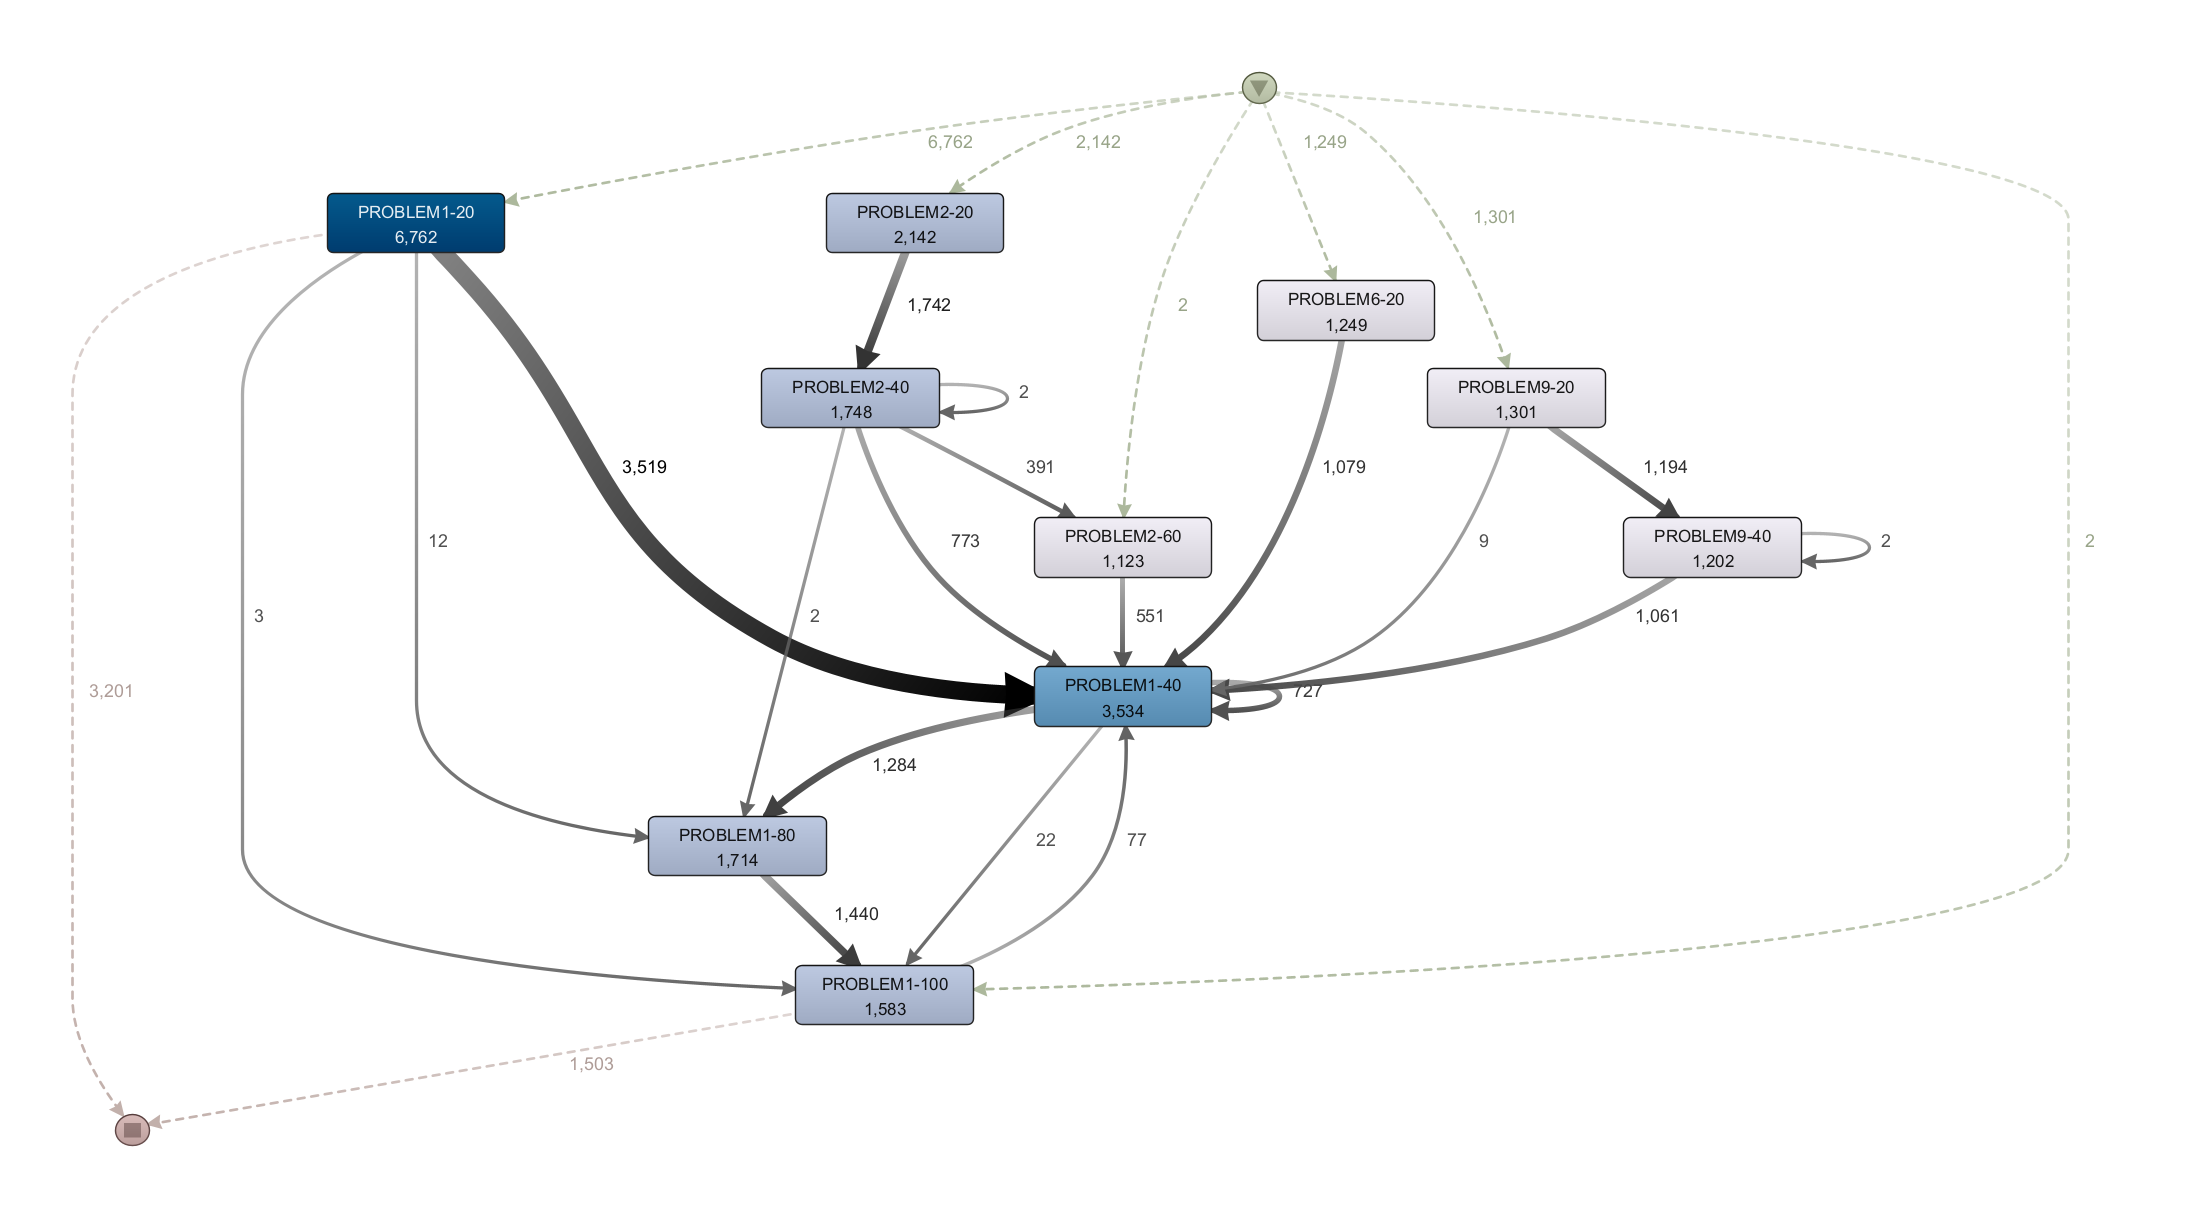
\includegraphics[width=1.25\textwidth]{imagenes/DISCO_compound/Dataset Fusionado - Compuesto.png}
    \caption{Análisis de procesos del dataset compuesto (acción compuesta).}
    \label{fig:datasetFusionadoCompuesto}
\end{figure}

\subsection{Segmentación por años}

\begin{figure}[H]
  \begin{subfigure}[t]{0.60\textwidth}
    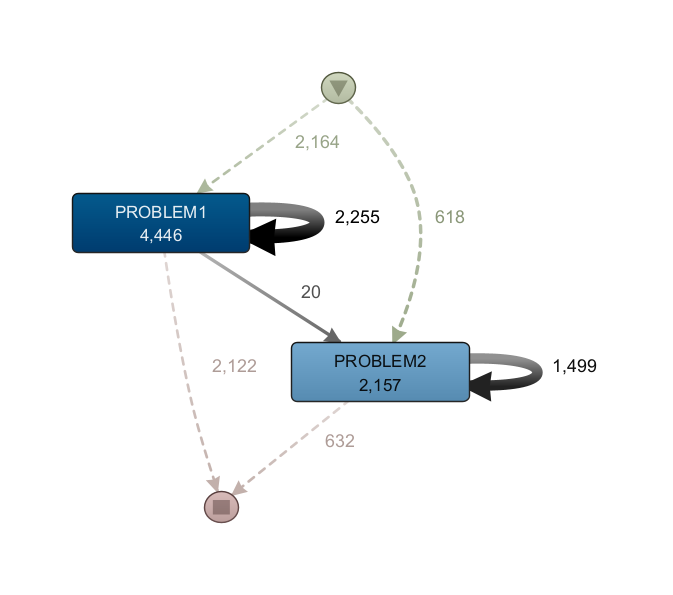
\includegraphics[width=1.10\textwidth, height=1.10\textwidth]{imagenes/DISCO_map/Dataset FusionadoYear1516.png}
    \caption{Extracción de procesos del curso académico 1516 (acción mapa).}
    \label{fig:mapAño1516}
  \end{subfigure}
  \hfill
  \begin{subfigure}[t]{0.60\textwidth}
    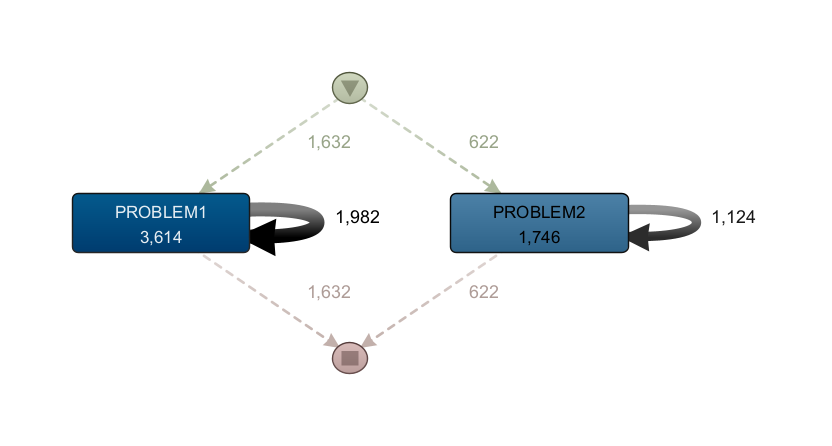
\includegraphics[width=1.10\textwidth, height=0.80\textwidth]{imagenes/DISCO_map/Dataset FusionadoYear1617.png}
    \caption{Extracción de procesos del curso académico 1617 (acción mapa).}
    \label{fig:mapAño1617}
  \end{subfigure}
  \hfill
  \begin{subfigure}[t]{0.60\textwidth}
    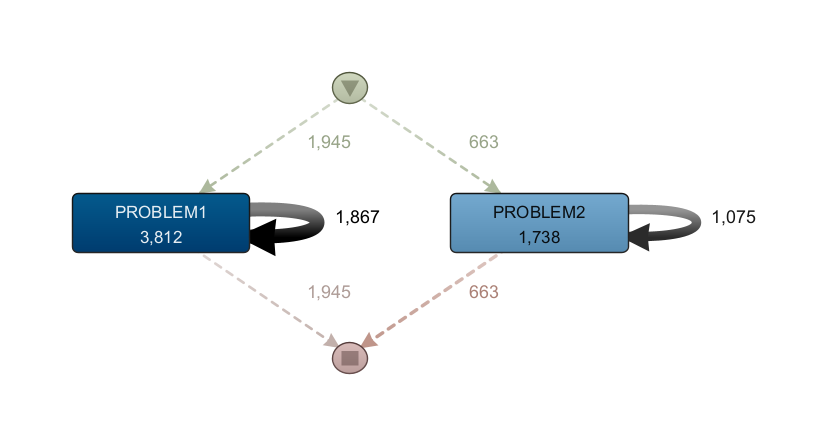
\includegraphics[width=1.10\textwidth, height=0.80\textwidth]{imagenes/DISCO_map/Dataset FusionadoYear1718.png}
    \caption{Extracción de procesos del curso académico 1718 (acción mapa).}
    \label{fig:mapAño1718}
  \end{subfigure}
  \hfill
  \begin{subfigure}[t]{0.60\textwidth}
    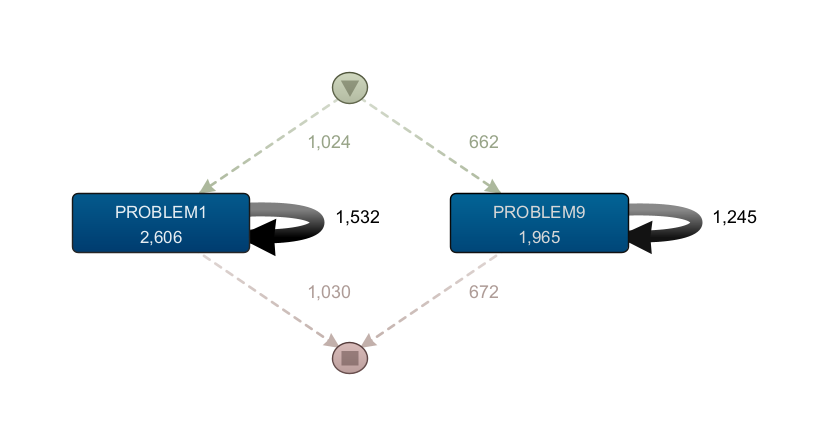
\includegraphics[width=1.10\textwidth, height=0.80\textwidth]{imagenes/DISCO_map/Dataset FusionadoYear1920.png}
    \caption{Extracción de procesos del curso académico 1920 (acción mapa).}
    \label{fig:mapAño1920}
  \end{subfigure}
  \caption{Extracción de procesos de los diferentes cursos académicos (acción mapa/problema).}
\end{figure}

Como puede observarse, mientras que en los cursos académicos 1516, 1617 y 1718 predominan los problemas $1$ y $2$, en el curso académico lo hacen los problemas $1$ y $9$. Esto refleja que los alumnos del curso escolar 1920 se tomaron gran interés en intentar resolver el noveno y más difícil de los problemas.

\begin{figure}[H]
    \centering
    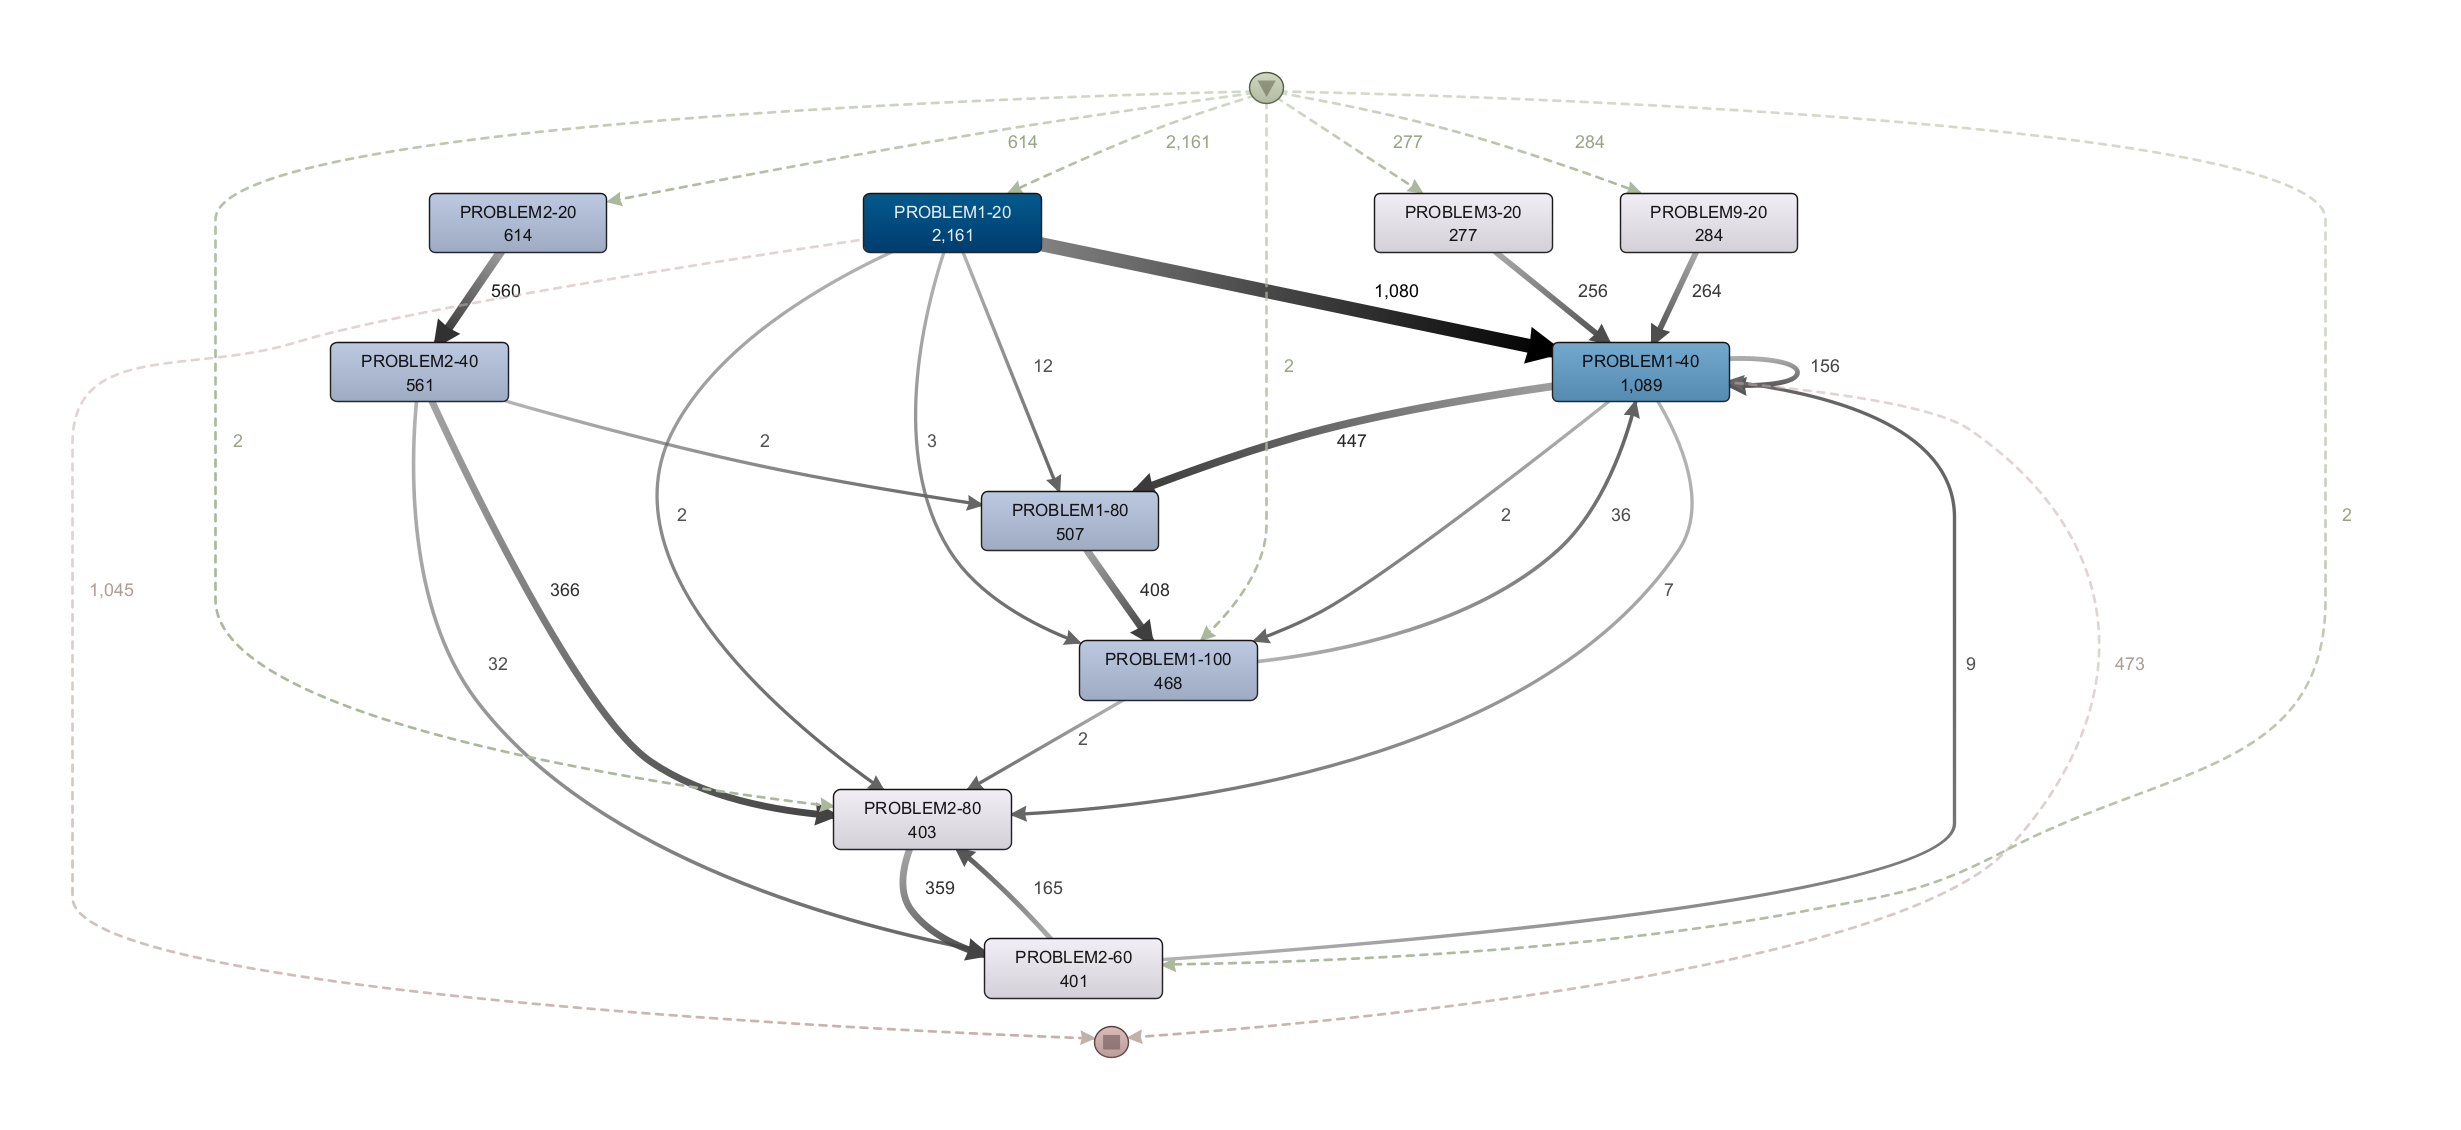
\includegraphics[width=1.25\textwidth]{imagenes/DISCO_compound/Year1516.png}
    \caption{Extracción de procesos del curso académico 1516 (acción compuesta).}
    \label{fig:año1516}
\end{figure}

\begin{figure}[H]
    \centering
    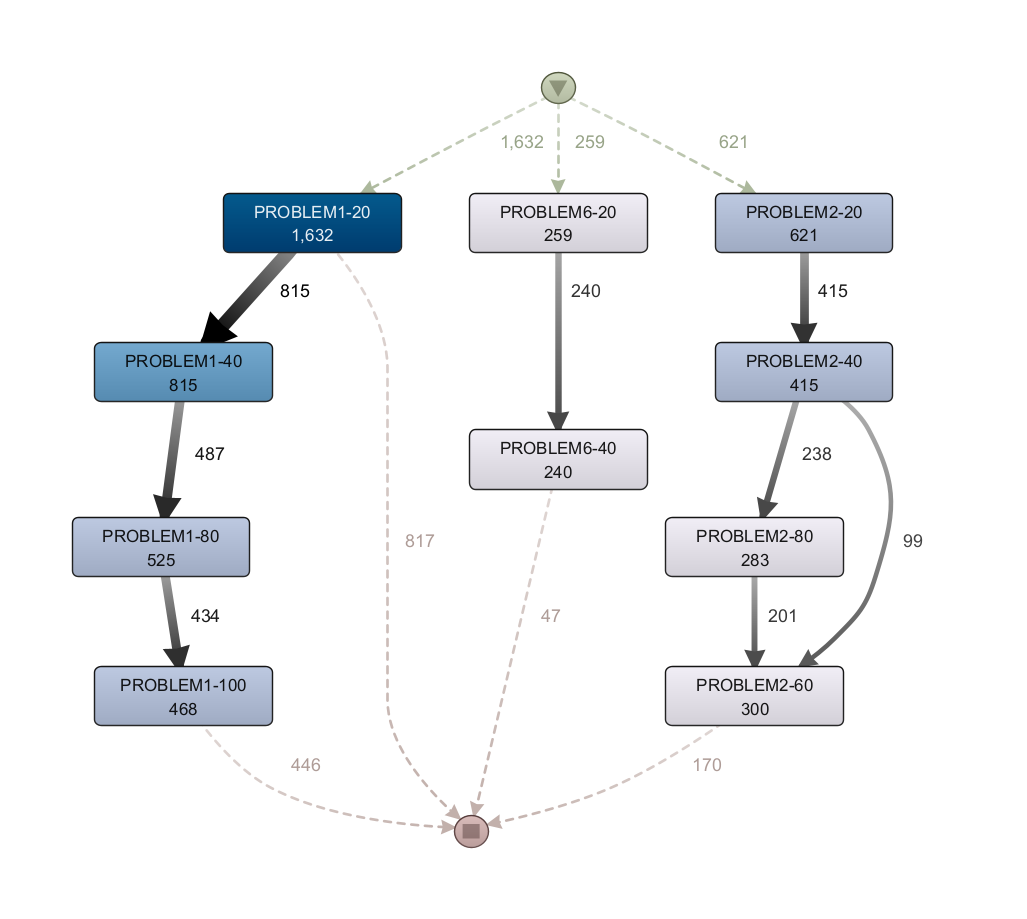
\includegraphics[width=1.25\textwidth]{imagenes/DISCO_compound/Year1617.png}
    \caption{Extracción de procesos del curso académico 1617 (acción compuesta).}
    \label{fig:año1617}
\end{figure}

\begin{figure}[H]
    \centering
    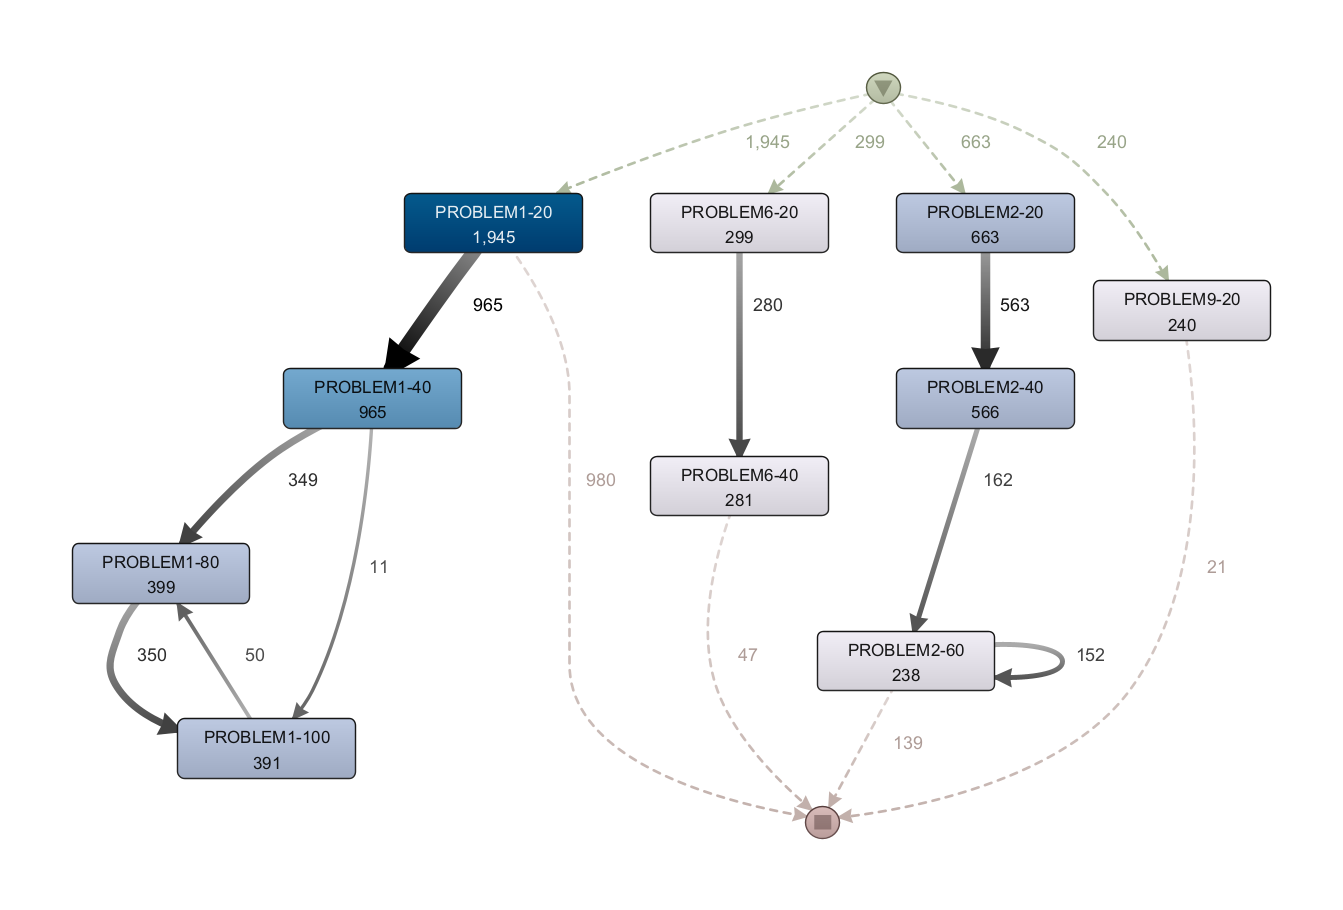
\includegraphics[width=1.25\textwidth]{imagenes/DISCO_compound/Year1718.png}
    \caption{Extracción de procesos del curso académico 1718 (acción compuesta).}
    \label{fig:año1718}
\end{figure}

\begin{figure}[H]
    \centering
    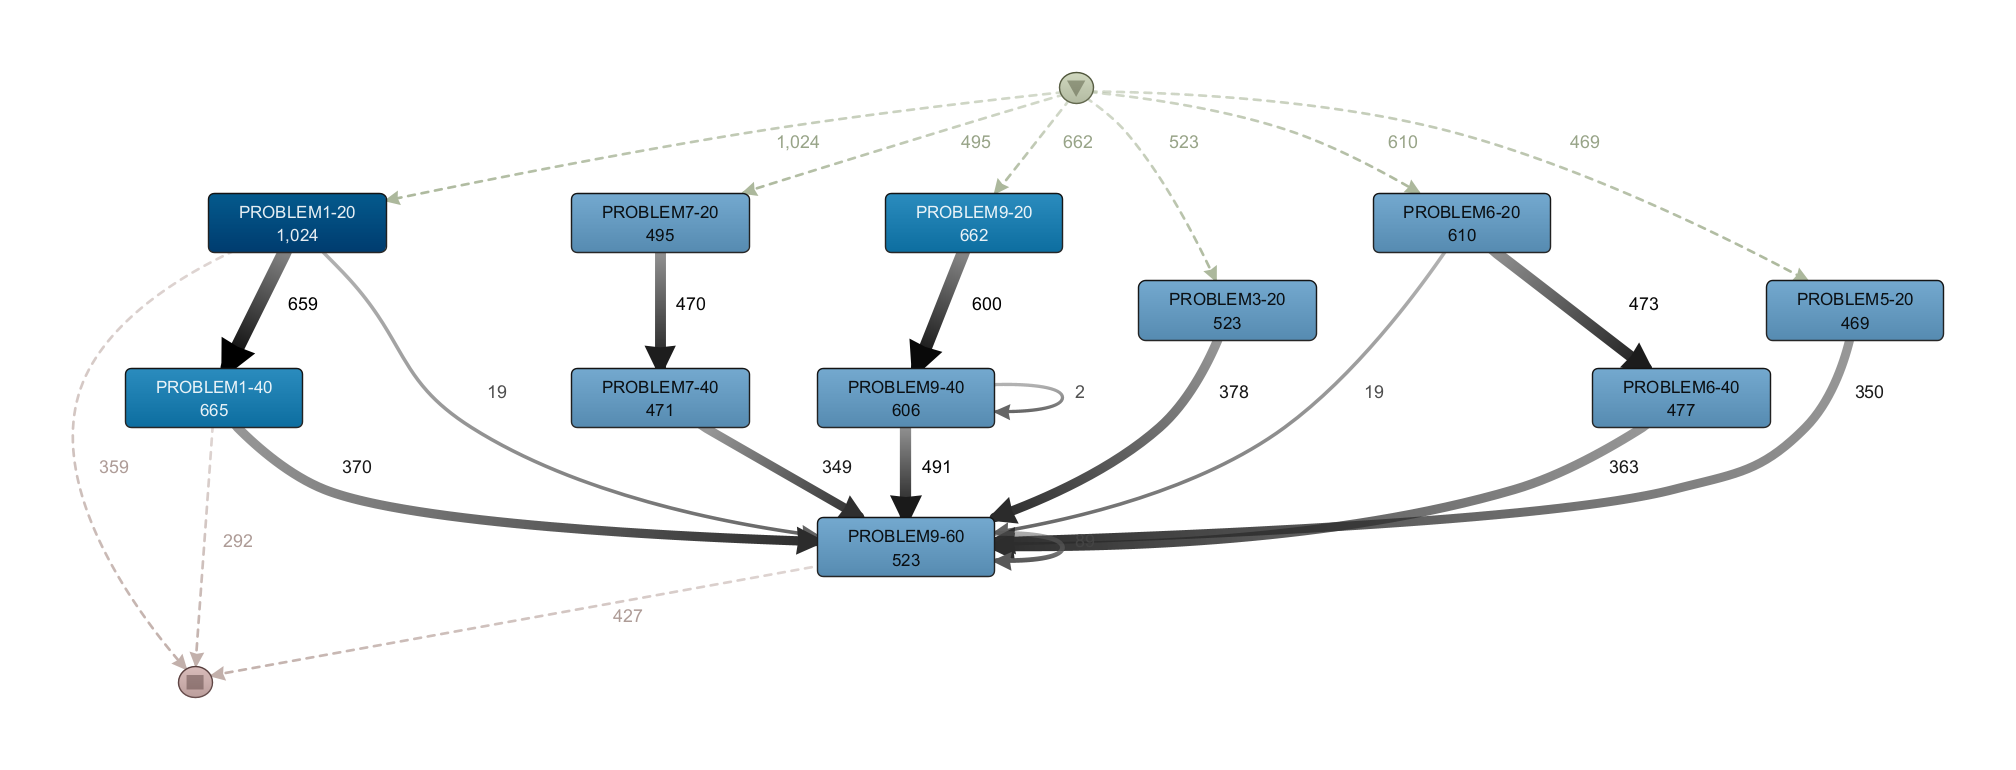
\includegraphics[width=1.25\textwidth]{imagenes/DISCO_compound/Year1920.png}
    \caption{Extracción de procesos del curso académico 1920 (acción compuesta).}
    \label{fig:año1920}
\end{figure}

Como podemos observar en la Figura \ref{fig:año1920}, los procesos extraídos en el curso académico 1920 resultan ser algo distintos a los del resto de cursos, pues parece que hay un mayor variedad, habiendo nodos de hasta seis problemas diferentes y estando estos más balanceados.

\subsection{Segmentación por calificaciones}

De ahora en adelante se considerará que la calificación de un grupo es \emph{``baja''} si es inferior a $7.5$, \emph{``media-baja''} si es igual o mayor que $7.5$ y menor a $8.5$, \emph{``media-alta''} si es igual a o mayor que $8.5$ e inferior a $9.5$ y \emph{``alta''} si es igual o superior a $9.5$.

\begin{figure}[H]
  \begin{subfigure}[t]{0.60\textwidth}
    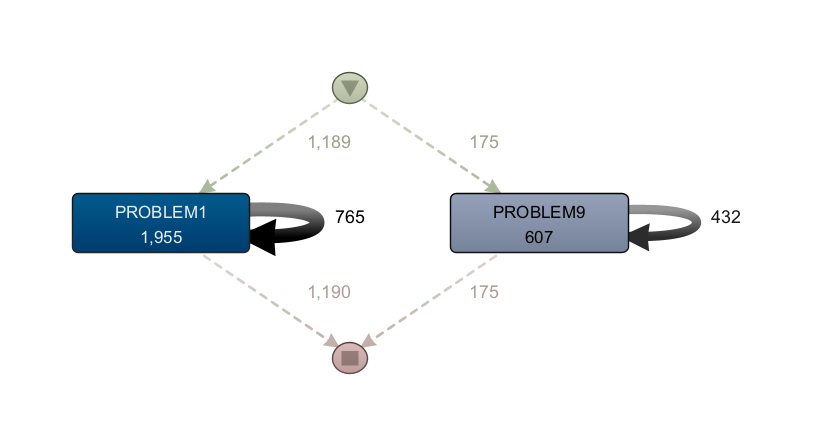
\includegraphics[width=1.10\textwidth, height=0.80\textwidth]{imagenes/DISCO_map/Dataset FusionadoWorstGrades.png}
    \caption{Extracción de procesos del dataset integrado por las acciones mapa de los grupos con calificación \emph{``baja''}.}
    \label{fig:mapWorstGrades}
  \end{subfigure}
  \hfill
  \begin{subfigure}[t]{0.60\textwidth}
    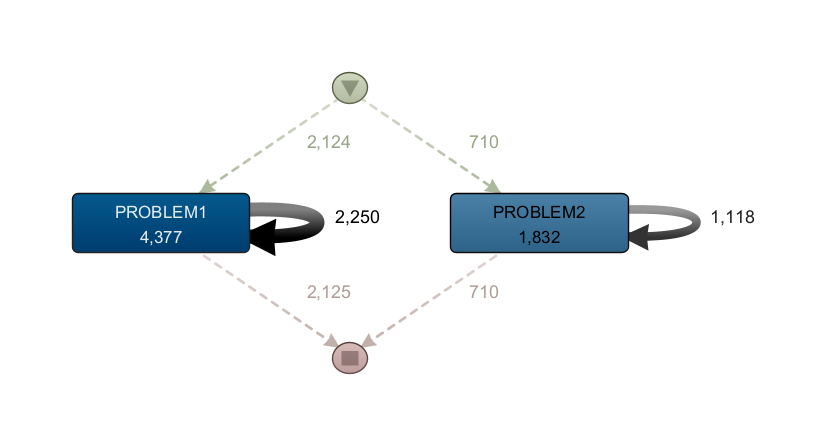
\includegraphics[width=1.10\textwidth, height=0.80\textwidth]{imagenes/DISCO_map/Dataset FusionadoMidLowGrades.png}
    \caption{Extracción de procesos del dataset integrado por las acciones mapa de los grupos con calificación \emph{``media-baja''}.}
    \label{fig:mapMidLowGrades}
  \end{subfigure}
  \hfill
  \begin{subfigure}[t]{0.60\textwidth}
    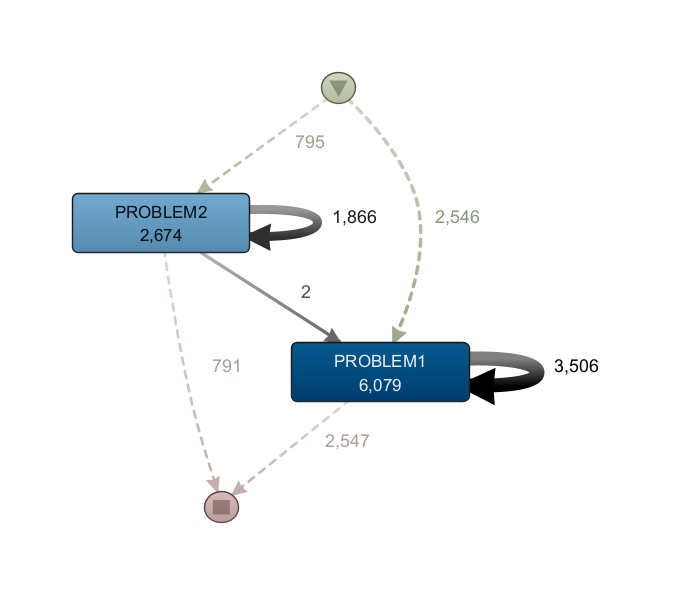
\includegraphics[width=1.10\textwidth, height=1.10\textwidth]{imagenes/DISCO_map/Dataset FusionadoMidHighGrades.png}
    \caption{Extracción de procesos del dataset integrado por las acciones mapa de los grupos con calificación \emph{``media-alta''}.}
    \label{fig:mapMidHighGrades}
  \end{subfigure}
  \hfill
  \begin{subfigure}[t]{0.60\textwidth}
    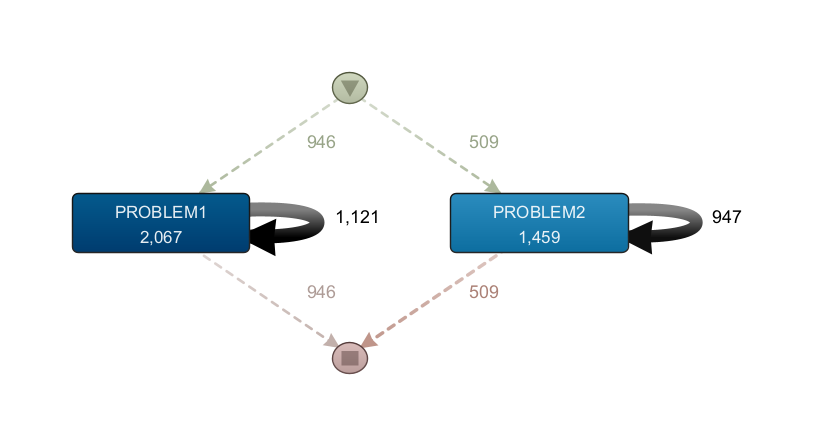
\includegraphics[width=1.10\textwidth, height=0.80\textwidth]{imagenes/DISCO_map/Dataset FusionadoHighGrades.png}
    \caption{Extracción de procesos del dataset integrado por las acciones mapa de los grupos con calificación \emph{``alta''}.}
    \label{fig:mapHighGrades}
  \end{subfigure}
  \caption{Extracción de procesos del dataset integrado por las acciones mapa de los grupos según sus calificaciones.}
\end{figure}

Tras haber extraído los correspondientes grafos, notamos que los grupos con calificación \emph{``baja''} han frecuentado más los problemas $1$ y $9$ mientras que los problemas más visitados por el resto de grupos son el $1$ y el $2$. Esto puede sugerir los grupos con ``peor'' calificación no han frecuentado lo suficiente los problemas de menor dificultad y, por el contrario, han intentado resolver la más difícil de las pruebas.

\begin{figure}[H]
    \centering
    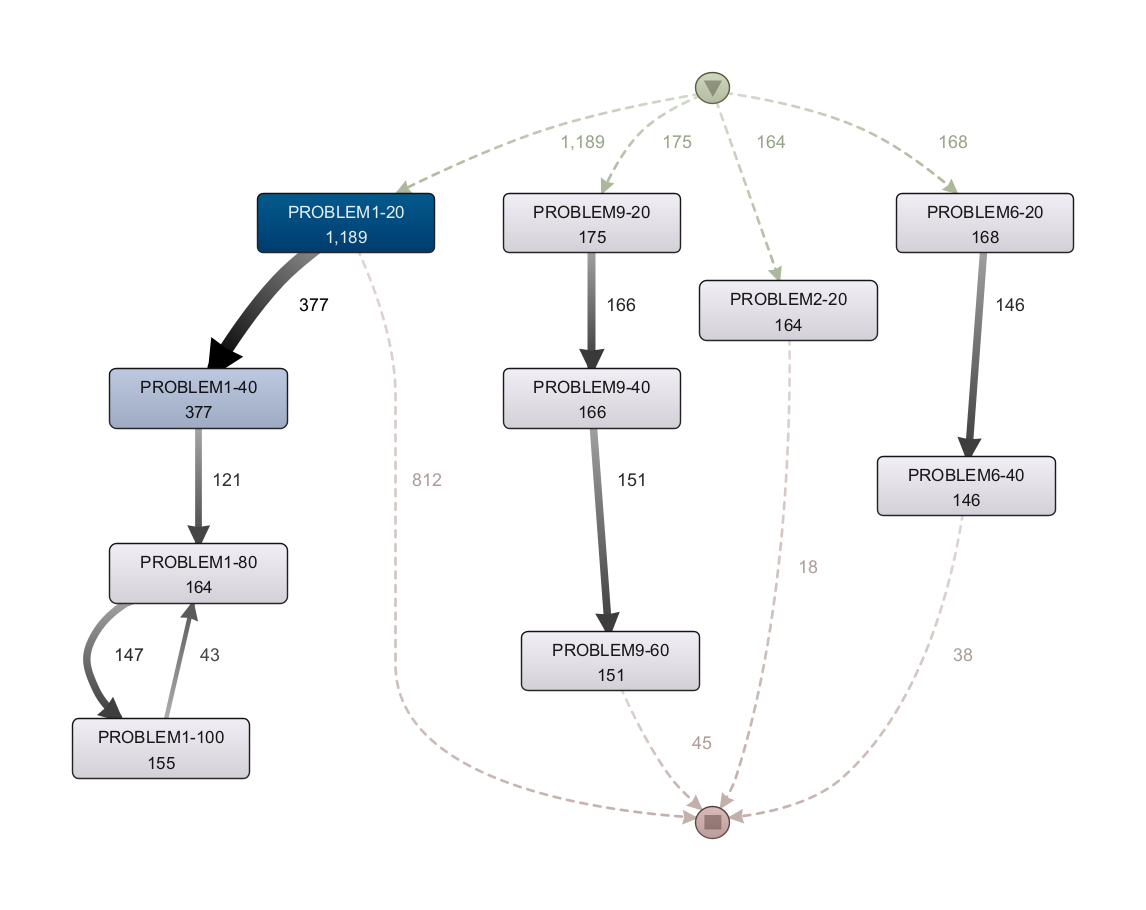
\includegraphics[width=1.25\textwidth]{imagenes/DISCO_compound/WorstGrades.png}
    \caption{Extracción de procesos del dataset integrado por las acciones compuestas de los grupos con calificación \emph{``baja''}.}
    \label{fig:worstGrades}
\end{figure}

\begin{figure}[H]
    \centering
    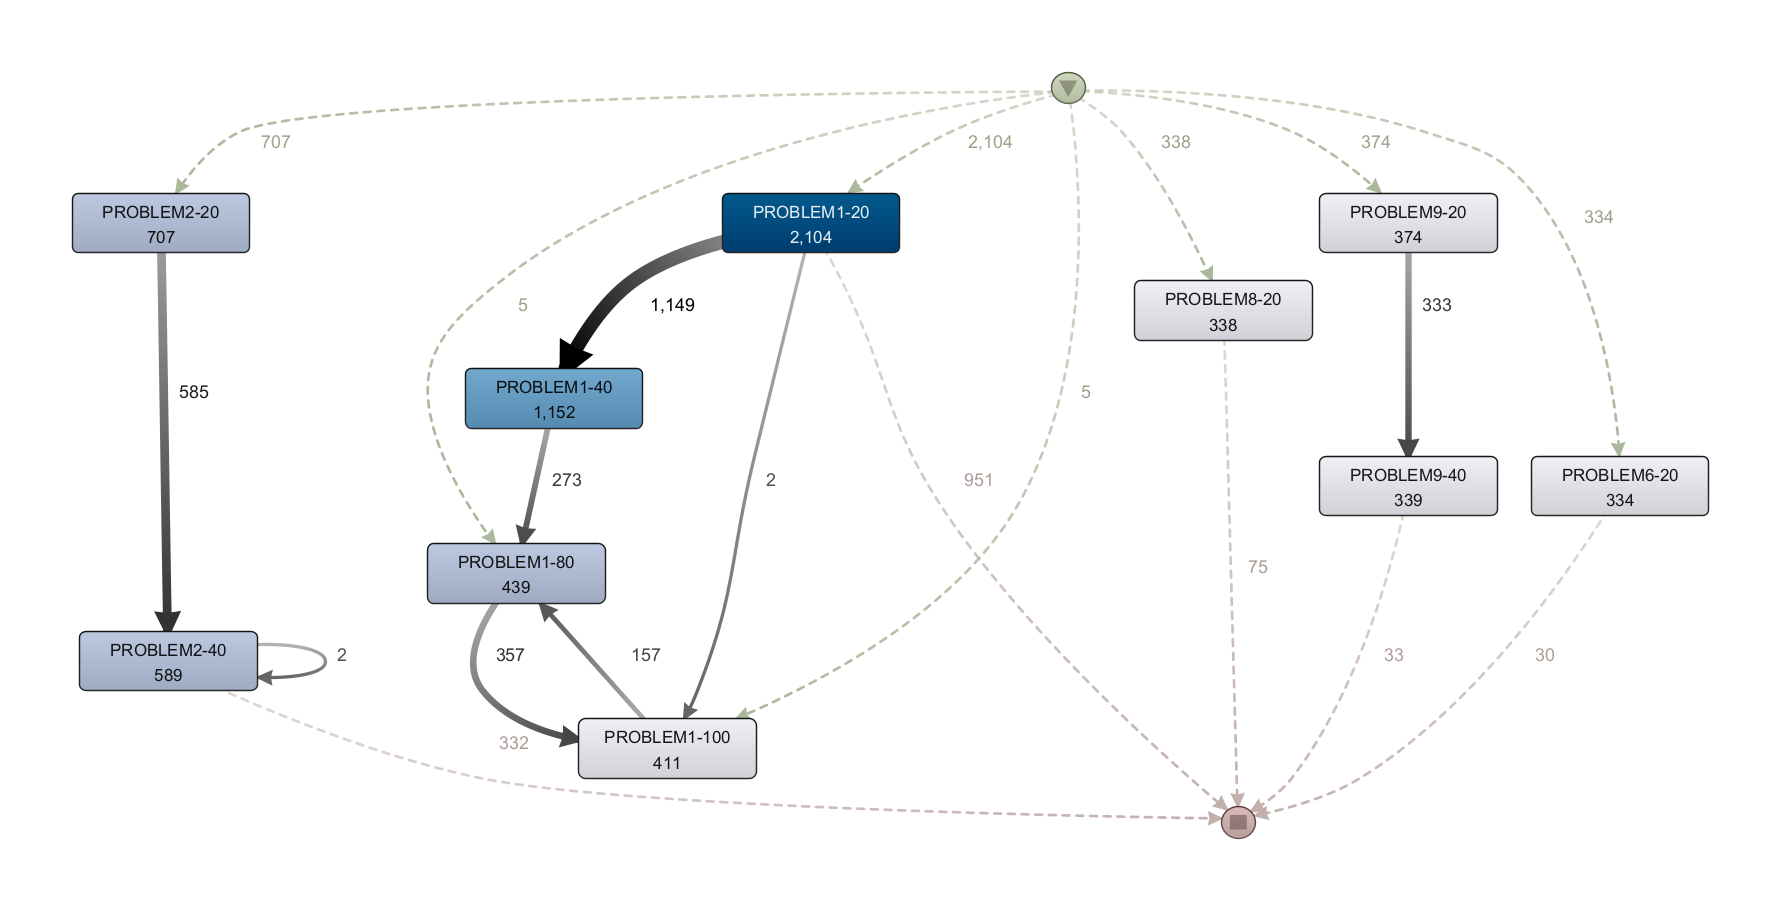
\includegraphics[width=1.25\textwidth]{imagenes/DISCO_compound/MidLowGrades.png}
    \caption{Extracción de procesos del dataset integrado por las acciones compuestas de los grupos con calificación \emph{``media-baja''}.}
    \label{fig:midLowGrades}
\end{figure}

\begin{figure}[H]
    \centering
    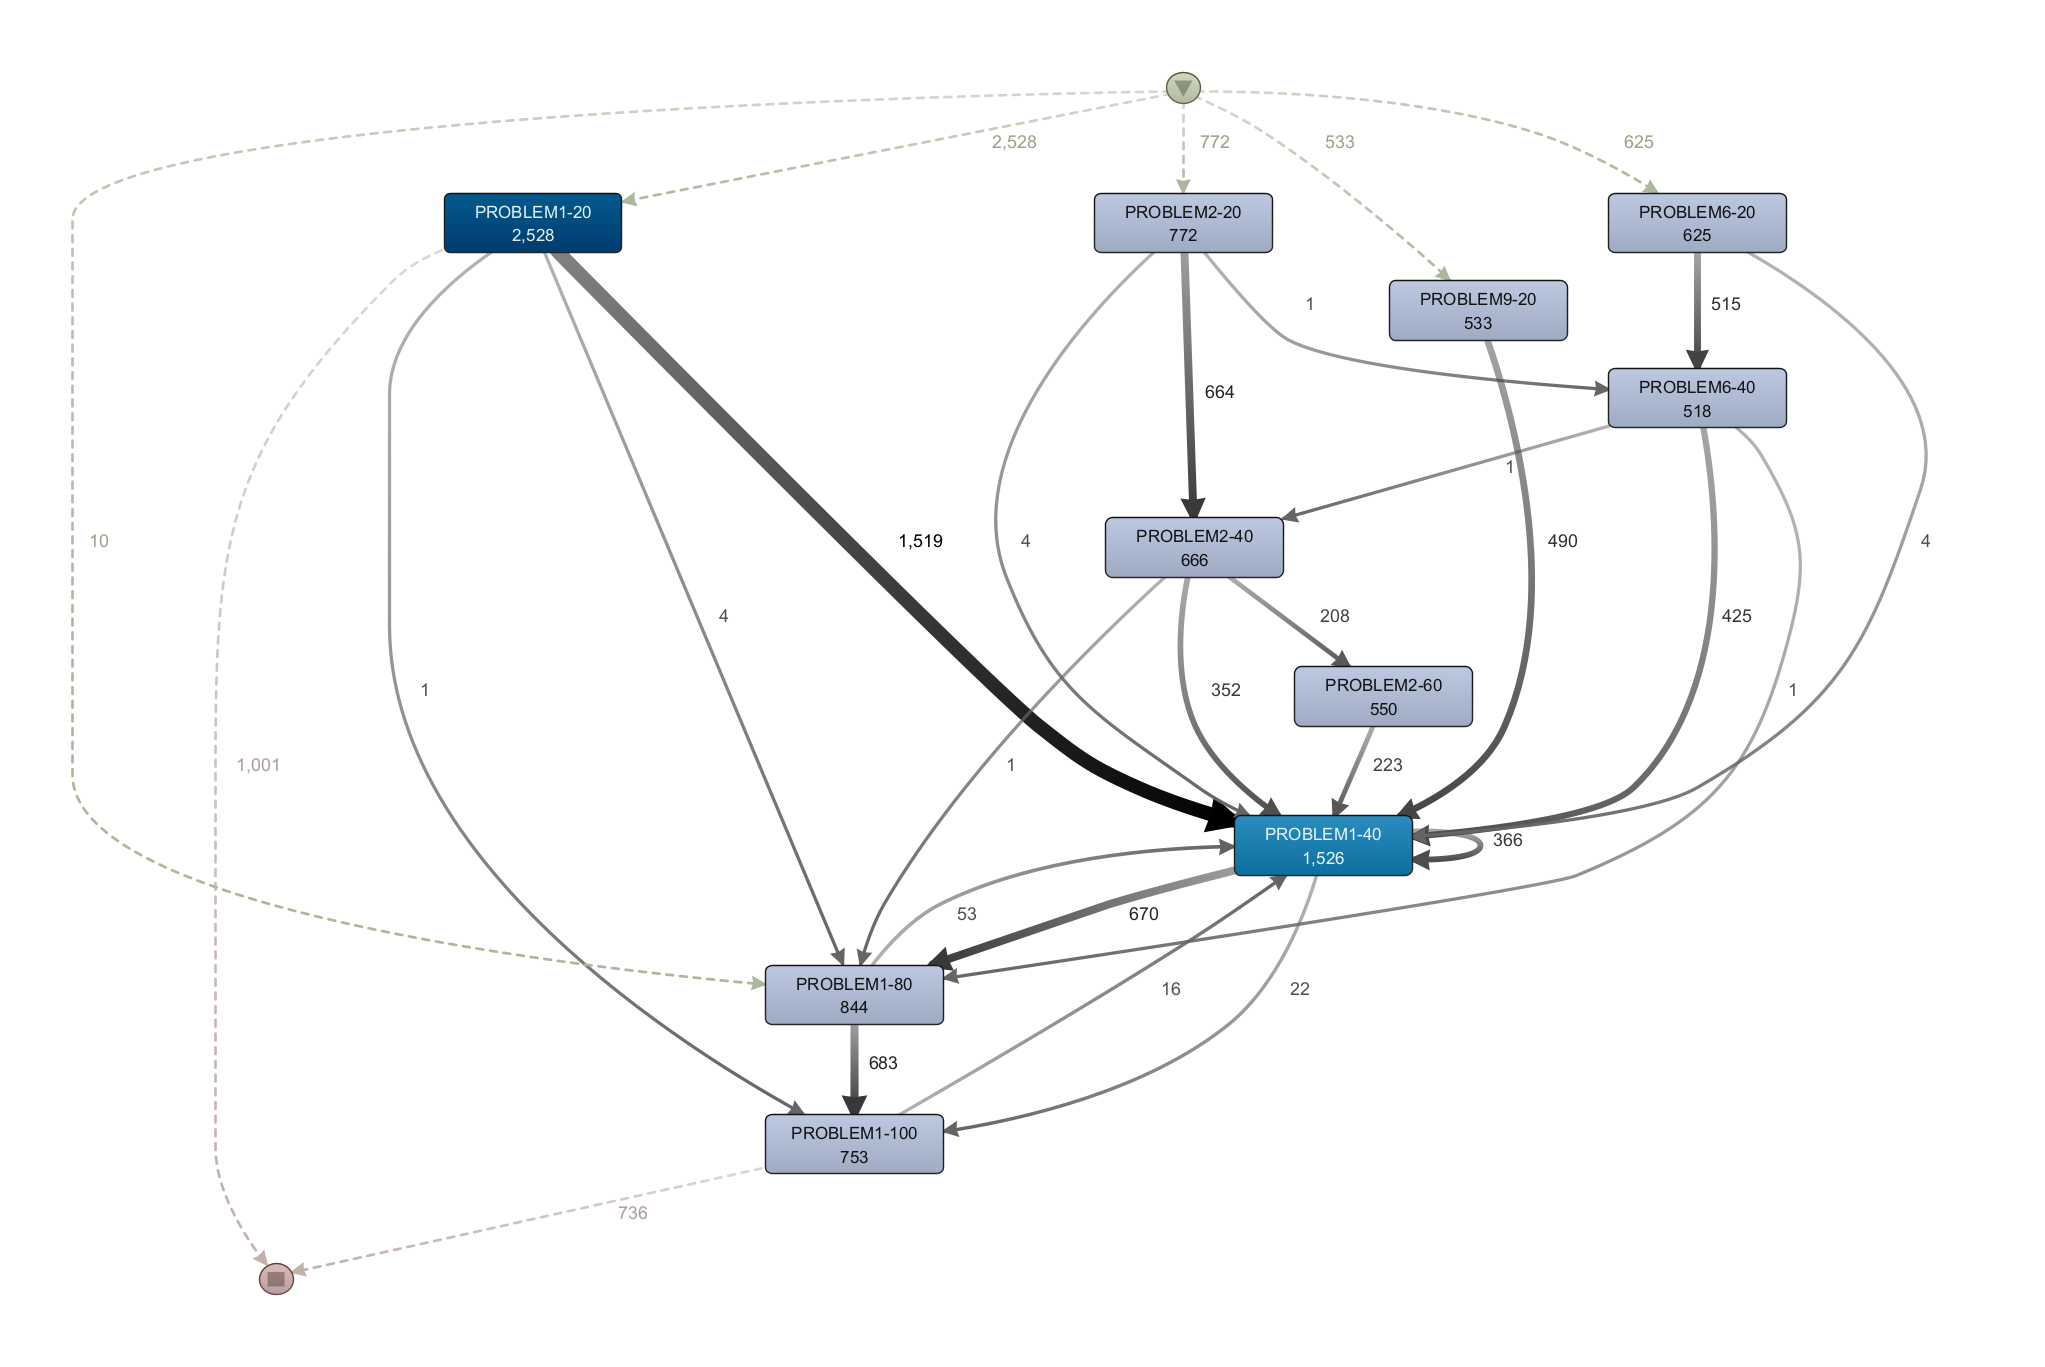
\includegraphics[width=1.25\textwidth]{imagenes/DISCO_compound/MidHighGrades.png}
    \caption{Extracción de procesos del dataset integrado por las acciones compuestas de los grupos con calificación \emph{``media-alta''}.}
    \label{fig:midHighGrades}
\end{figure}

\begin{figure}[H]
    \centering
    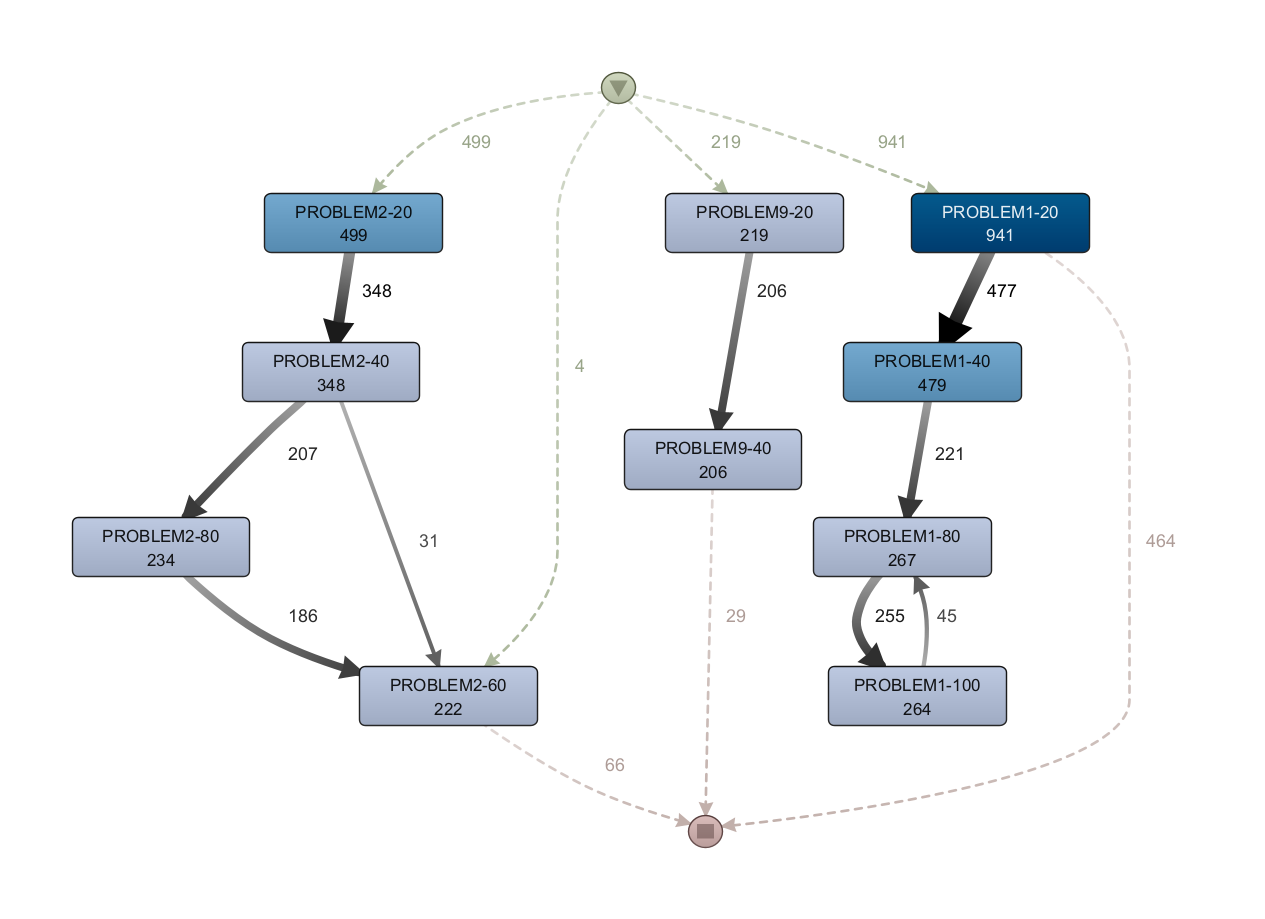
\includegraphics[width=1.25\textwidth]{imagenes/DISCO_compound/BestGrades.png}
    \caption{Extracción de procesos del dataset integrado por las acciones compuestas de los grupos con calificación \emph{``alta''}.}
    \label{fig:bestGrades}
\end{figure}

Observando las Figuras \ref{fig:worstGrades}, \ref{fig:midLowGrades}, \ref{fig:midHighGrades} y \ref{fig:bestGrades}, podemos ver que hay una correlación directa de la nota que sacan con la frecuencia relativa del problema con la que frecuence el nodo \texttt{PROBLEM2-20}.

\subsection{Segmentación por año y calificación}

\begin{figure}[H]
  \begin{subfigure}[t]{0.60\textwidth}
    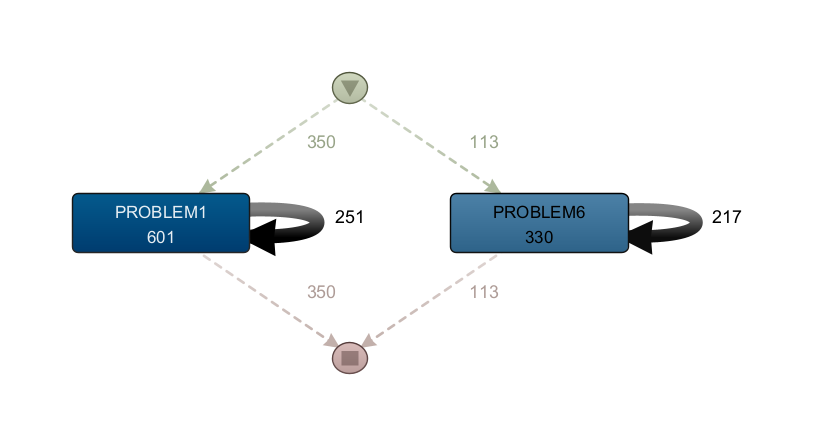
\includegraphics[width=1.10\textwidth, height=0.80\textwidth]{imagenes/DISCO_map/Dataset FusionadoYear1617WorstGrades.png}
    \caption{Extracción de procesos del dataset integrado por las acciones mapa de los grupos con calificación \emph{``baja''} del curso académico 1617.}
    \label{fig:mapYear1617WorstGrades}
  \end{subfigure}
  \hfill
  \begin{subfigure}[t]{0.60\textwidth}
    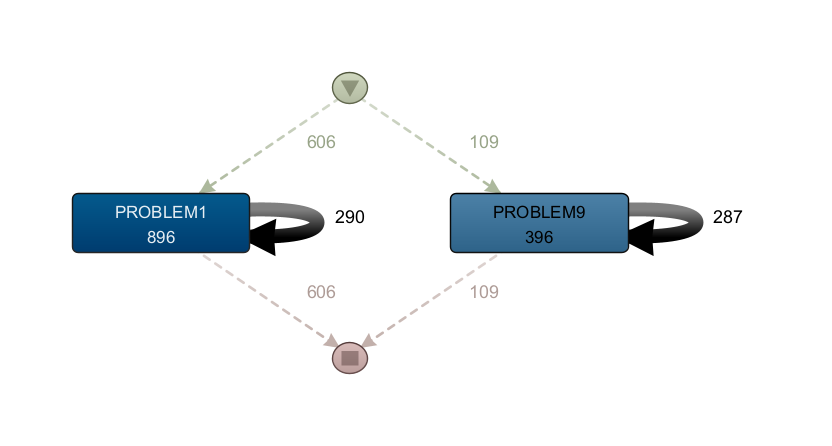
\includegraphics[width=1.10\textwidth, height=0.80\textwidth]{imagenes/DISCO_map/Dataset FusionadoYear1718WorstGrades.png}
    \caption{Extracción de procesos del dataset integrado por las acciones mapa de los grupos con calificación \emph{``baja''} del curso académico 1718.}
    \label{fig:mapYear1718WorstGrades}
  \end{subfigure}
  \hfill
  \begin{subfigure}[t]{0.60\textwidth}
    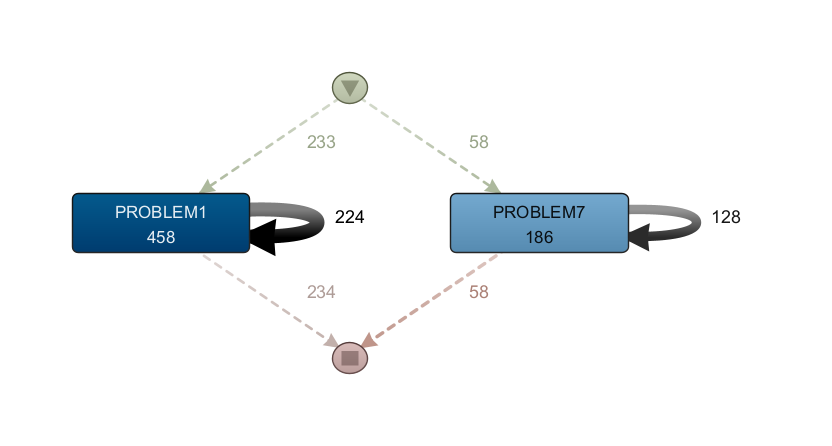
\includegraphics[width=1.10\textwidth, height=0.80\textwidth]{imagenes/DISCO_map/Dataset FusionadoYear1920WorstGrades.png}
    \caption{Extracción de procesos del dataset integrado por las acciones mapa de los grupos con calificación \emph{``baja''} del curso académico 1920.}
    \label{fig:mapYear1920WorstGrades}
  \end{subfigure}
  \caption{Extracción de procesos del dataset integrado por las acciones mapa de los grupos con calificación \emph{``baja''} a lo largo de cuatro cursos académicos.}
\end{figure}

Tal y como puede observarse en la Figura que se muestra anteriormente, los grupos con las peores calificaciones a lo largo de los cuatro cursos académicos tienden a emplear mucho tiempo en el problema $1$ y en otro problema con una numeración alta (en este caso, en el curso 1617 es el problema $6$, en el curso 1718 es el problema $9$ y en el 1920 es el problema $7$). Esto podría indicar que no prestan demasiada atención a resolver problemas más fáciles, intentando resolver los más difíciles a lo mejor sin los conocimientos o la base necesaria. No obstante, también podría haber ocurrido que esos problemas en particular hubieran sido un quebradero de cabeza para esos grupos en esos cursos. Así pues, podrían haberse quedado atascados y haber invertido muchos más recursos en esos problemas que en el resto.

\begin{figure}[H]
  \begin{subfigure}[t]{0.60\textwidth}
    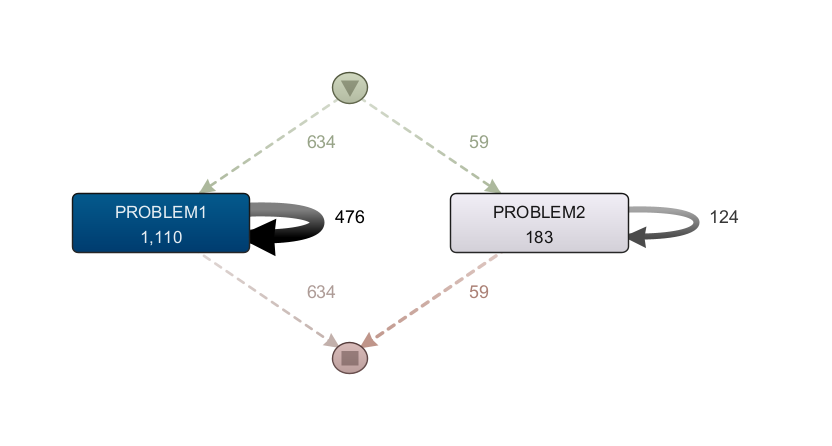
\includegraphics[width=1.10\textwidth, height=0.80\textwidth]{imagenes/DISCO_map/Dataset FusionadoYear1516MidLowGrades.png}
    \caption{Extracción de procesos del dataset integrado por las acciones mapa de los grupos con calificación \emph{``media-baja''} del curso académico 1516.}
    \label{fig:mapYear1516MidLowGrades}
  \end{subfigure}
  \hfill
  \begin{subfigure}[t]{0.60\textwidth}
    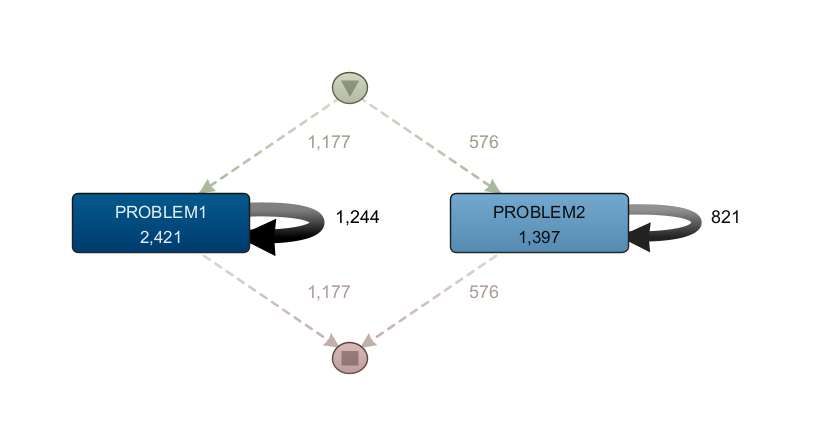
\includegraphics[width=1.10\textwidth, height=0.80\textwidth]{imagenes/DISCO_map/Dataset FusionadoYear1718MidLowGrades.png}
    \caption{Extracción de procesos del dataset integrado por las acciones mapa de los grupos con calificación \emph{``media-baja''} del curso académico 1718.}
    \label{fig:mapYear1718MidLowGrades}
  \end{subfigure}
  \hfill
  \begin{subfigure}[t]{0.60\textwidth}
    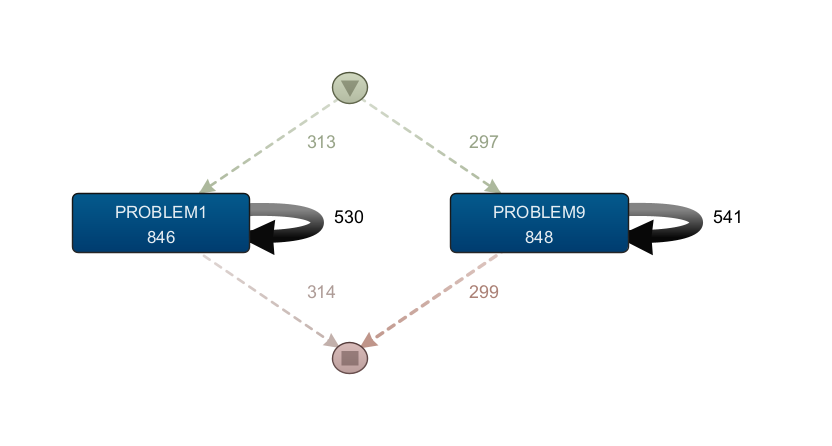
\includegraphics[width=1.10\textwidth, height=0.80\textwidth]{imagenes/DISCO_map/Dataset FusionadoYear1920MidLowGrades.png}
    \caption{Extracción de procesos del dataset integrado por las acciones mapa de los grupos con calificación \emph{``media-baja''} del curso académico 1920.}
    \label{fig:mapYear1920MidLowGrades}
  \end{subfigure}
  \caption{Extracción de procesos del dataset integrado por las acciones mapa de los grupos con calificación \emph{``media-baja''} a lo largo de cuatro cursos académicos.}
\end{figure}

Podemos observar que hay claras diferencias con respecto a la Figura anterior. Por ejemplo, en los cursos académicos 1516 y 1718 los problemas de numeración más baja (los problemas $1$ y $2$) sobresalen con las frecuencias más altas. Esto puede indicar que a lo mejor han resuelto los diferentes de manera más progresiva, sin lanzarse a resolver los problemas más difíciles desde el principio. Sin embargo, en el curso académico 1920 todavía podemos observar aún lo mencionado en los grafos de los procesos extraídos de los grupos de alumnos con calificación \emph{``baja''}.

\begin{figure}[H]
  \begin{subfigure}[t]{0.60\textwidth}
    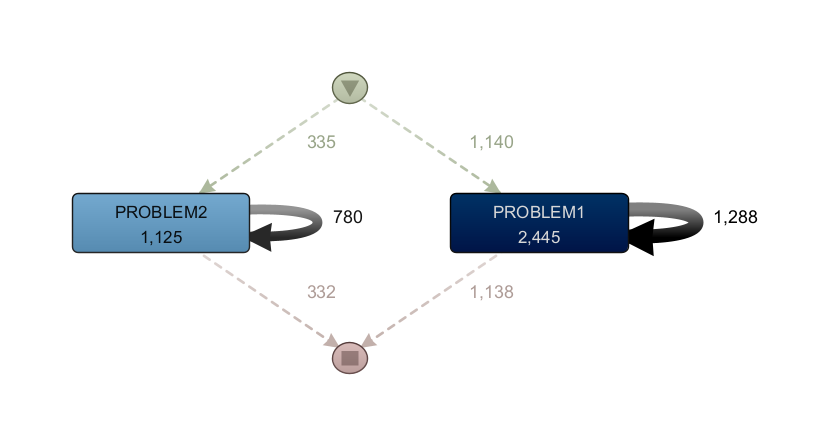
\includegraphics[width=1.10\textwidth, height=0.80\textwidth]{imagenes/DISCO_map/Dataset FusionadoYear1516MidHighGrades.png}
    \caption{Extracción de procesos del dataset integrado por las acciones mapa de los grupos con calificación \emph{``media-alta''} del curso académico 1516.}
    \label{fig:mapYear1516MidHighGrades}
  \end{subfigure}
  \hfill
  \begin{subfigure}[t]{0.60\textwidth}
    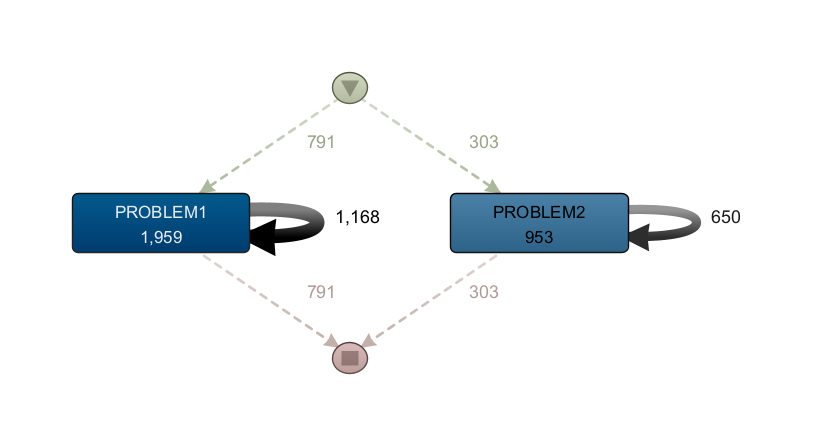
\includegraphics[width=1.10\textwidth, height=0.80\textwidth]{imagenes/DISCO_map/Dataset FusionadoYear1617MidHighGrades.png}
    \caption{Extracción de procesos del dataset integrado por las acciones mapa de los grupos con calificación \emph{``media-alta''} del curso académico 1617.}
    \label{fig:mapYear1617MidHighGrades}
  \end{subfigure}
  \hfill
  \begin{subfigure}[t]{0.60\textwidth}
    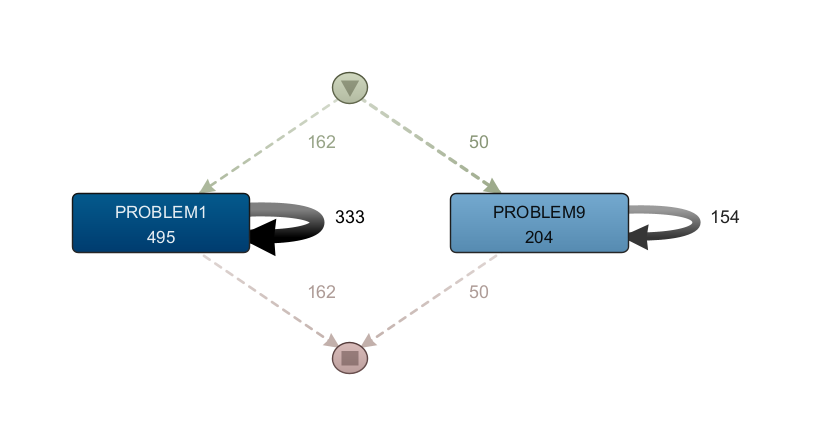
\includegraphics[width=1.10\textwidth, height=0.80\textwidth]{imagenes/DISCO_map/Dataset FusionadoYear1718MidHighGrades.png}
    \caption{Extracción de procesos del dataset integrado por las acciones mapa de los grupos con calificación \emph{``media-alta''} del curso académico 1718.}
    \label{fig:mapYear1718MidHighGrades}
  \end{subfigure}
  \hfill
  \begin{subfigure}[t]{0.60\textwidth}
    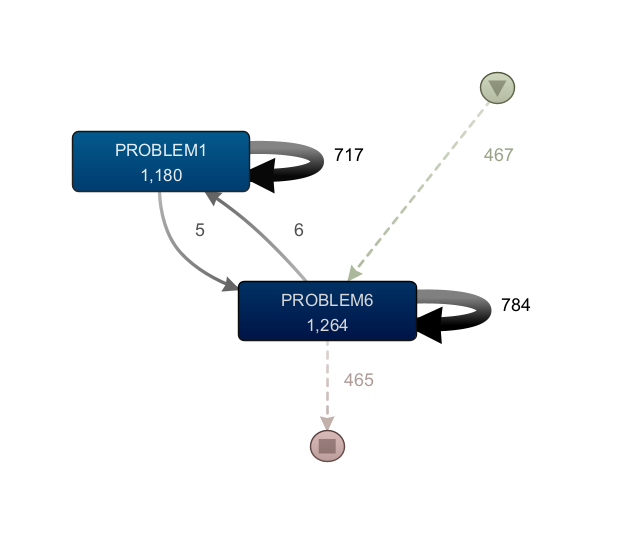
\includegraphics[width=1.10\textwidth, height=1.10\textwidth]{imagenes/DISCO_map/Dataset FusionadoYear1920MidHighGrades.png}
    \caption{Extracción de procesos del dataset integrado por las acciones mapa de los grupos con calificación \emph{``media-alta''} del curso académico 1920.}
    \label{fig:mapYear1920MidHighGrades}
  \end{subfigure}
  \caption{Extracción de procesos del dataset integrado por las acciones mapa de los grupos con calificación \emph{``media-alta''} a lo largo de cuatro cursos académicos.}
\end{figure}

En los grupos con calificación \emph{``media-alta''} podemos observar dos comportamientos diferentes. Por un lado, en los primeros cursos escolares (1617 y 1617) se sigue la tendencia de la Figura anterior, con la frecuencia de los problemas $1$ y $2$ predominando sobre las demás. Sin embargo, en el curso académico 1718, el segundo problema más frecuentado es el $9$ y en el curso académico 1920 el $6$ (siendo el problema $1$ el más visitado en ambos casos).

\begin{figure}[H]
  \begin{subfigure}[t]{0.60\textwidth}
    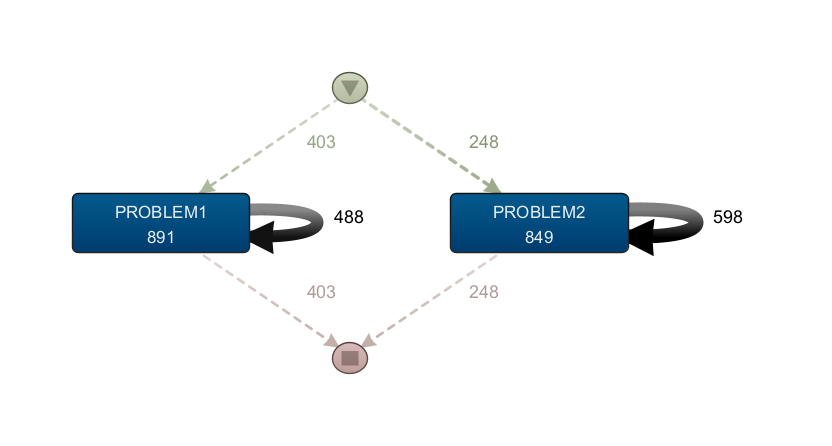
\includegraphics[width=1.10\textwidth, height=0.80\textwidth]{imagenes/DISCO_map/Dataset FusionadoYear1516HighGrades.png}
    \caption{Extracción de procesos del dataset integrado por las acciones mapa de los grupos con calificación \emph{``alta''} del curso académico 1516.}
    \label{fig:mapYear1516HighGrades}
  \end{subfigure}
  \hfill
  \begin{subfigure}[t]{0.60\textwidth}
    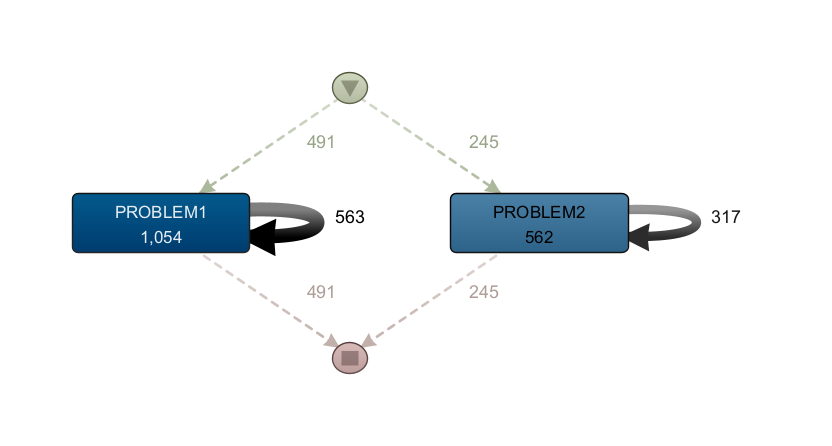
\includegraphics[width=1.10\textwidth, height=0.80\textwidth]{imagenes/DISCO_map/Dataset FusionadoYear1617HighGrades.png}
    \caption{Extracción de procesos del dataset integrado por las acciones mapa de los grupos con calificación \emph{``alta''} del curso académico 1617.}
    \label{fig:mapYear1617HighGrades}
  \end{subfigure}
  \hfill
  \begin{subfigure}[t]{0.60\textwidth}
    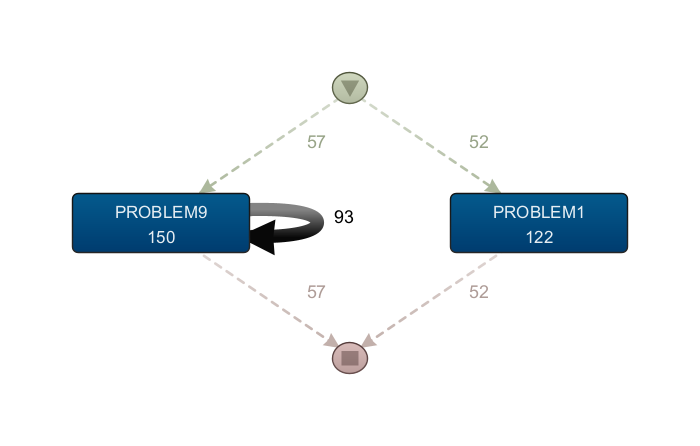
\includegraphics[width=1.10\textwidth, height=0.80\textwidth]{imagenes/DISCO_map/Dataset FusionadoYear1920HighGrades.png}
    \caption{Extracción de procesos del dataset integrado por las acciones mapa de los grupos con calificación \emph{``alta''} del curso académico 1920.}
    \label{fig:mapYear1920HighGrades}
  \end{subfigure}
  \caption{Extracción de procesos del dataset integrado por las acciones mapa de los grupos con calificación \emph{``alta''} a lo largo de cuatro cursos académicos.}
\end{figure}

El mismo patrón puede observarse en los grafos de los grupos con las calificaciones más altas en los cuatro cursos académicos, siendo los problemas $1$ y $9$ los más frecuentados en el curso 1920, mientras en el resto de los cursos son los problemas $1$ y $2$ los más frecuentados.

\begin{figure}[H]
    \centering
    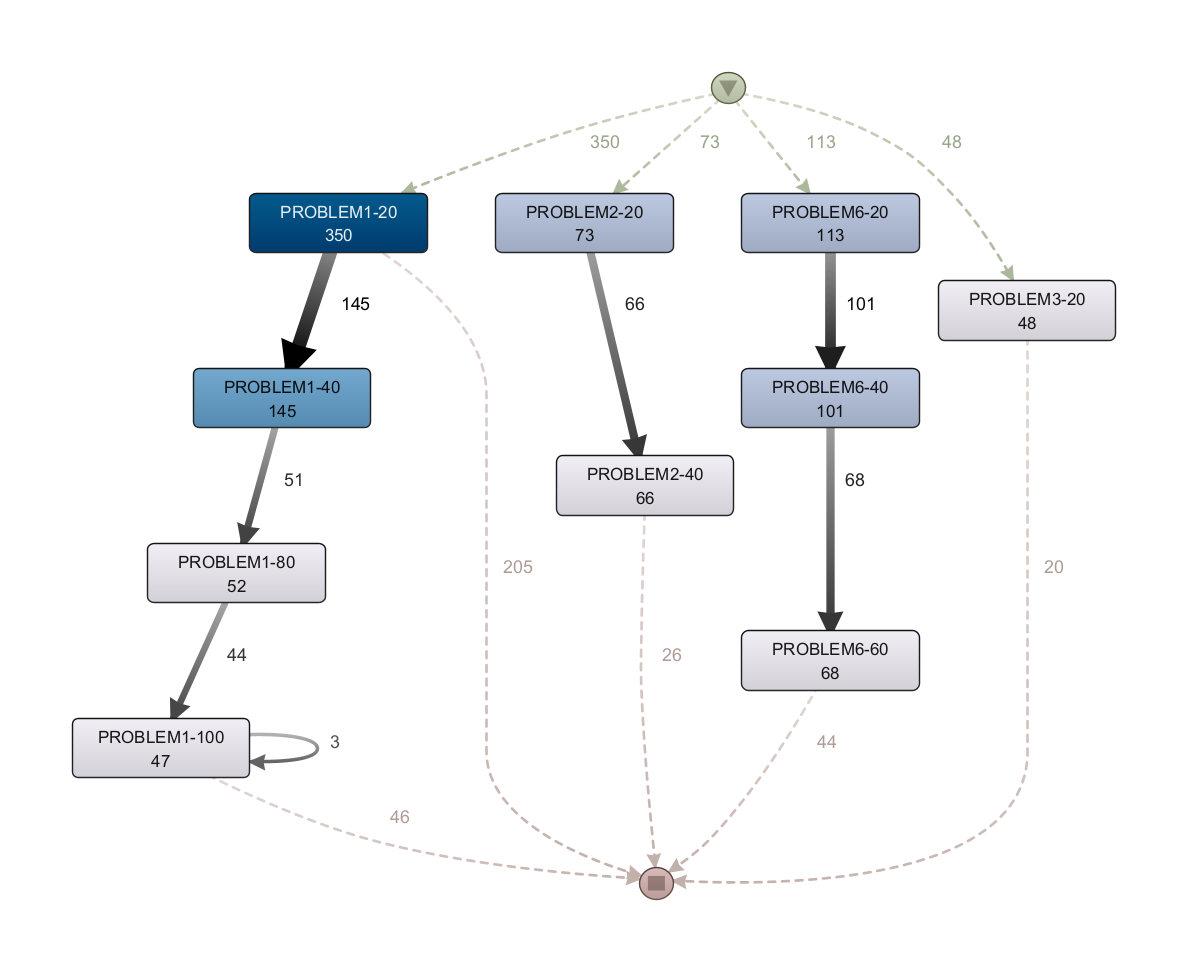
\includegraphics[width=1.25\textwidth]{imagenes/DISCO_compound/Year1617WorstGrades.png}
    \caption{Extracción de procesos del dataset integrado por las acciones compuestas de los grupos con calificación \emph{``baja''} del curso académico 1617.}
    \label{fig:year1617WorstGrades}
\end{figure}

\begin{figure}[H]
    \centering
    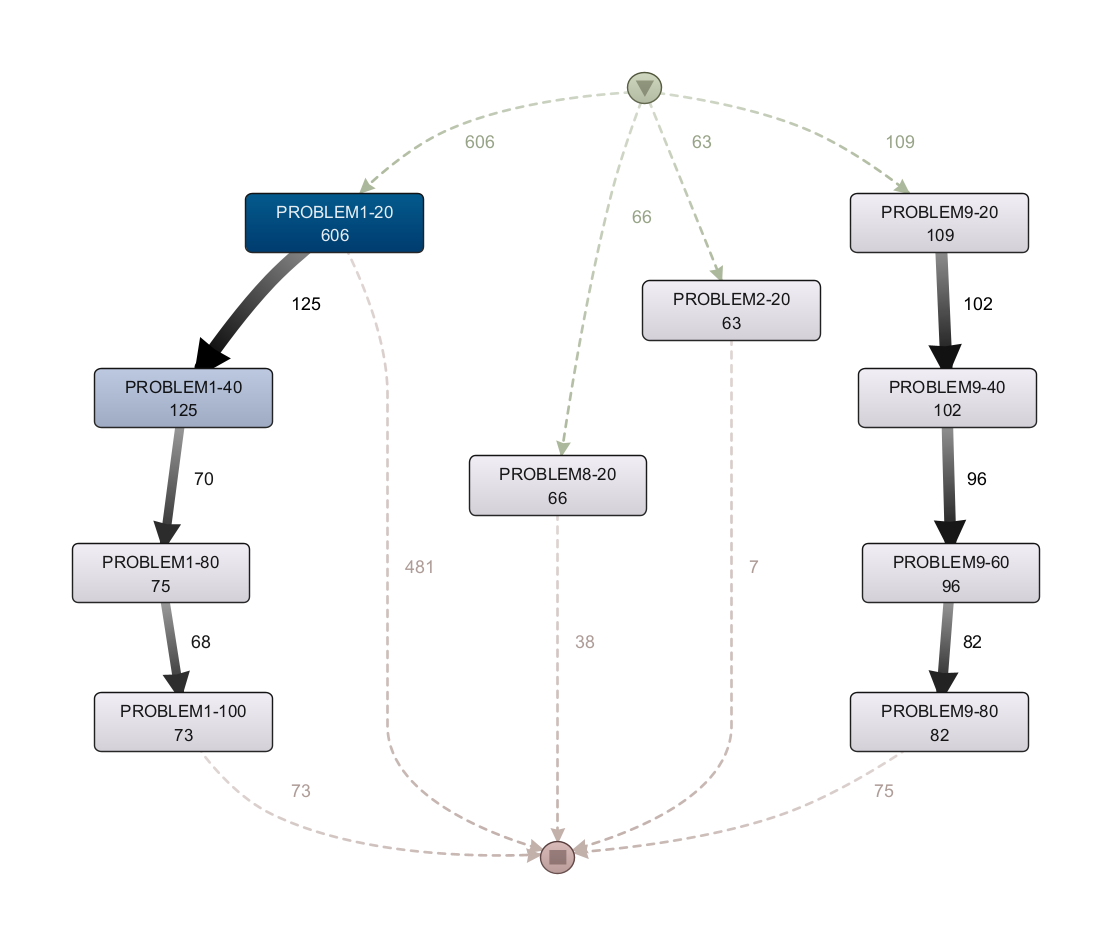
\includegraphics[width=1.25\textwidth]{imagenes/DISCO_compound/Year1718WorstGrades.png}
    \caption{Extracción de procesos del dataset integrado por las acciones compuestas de los grupos con calificación \emph{``baja''} del curso académico 1718.}
    \label{fig:year1718WorstGrades}
\end{figure}

\begin{figure}[H]
    \centering
    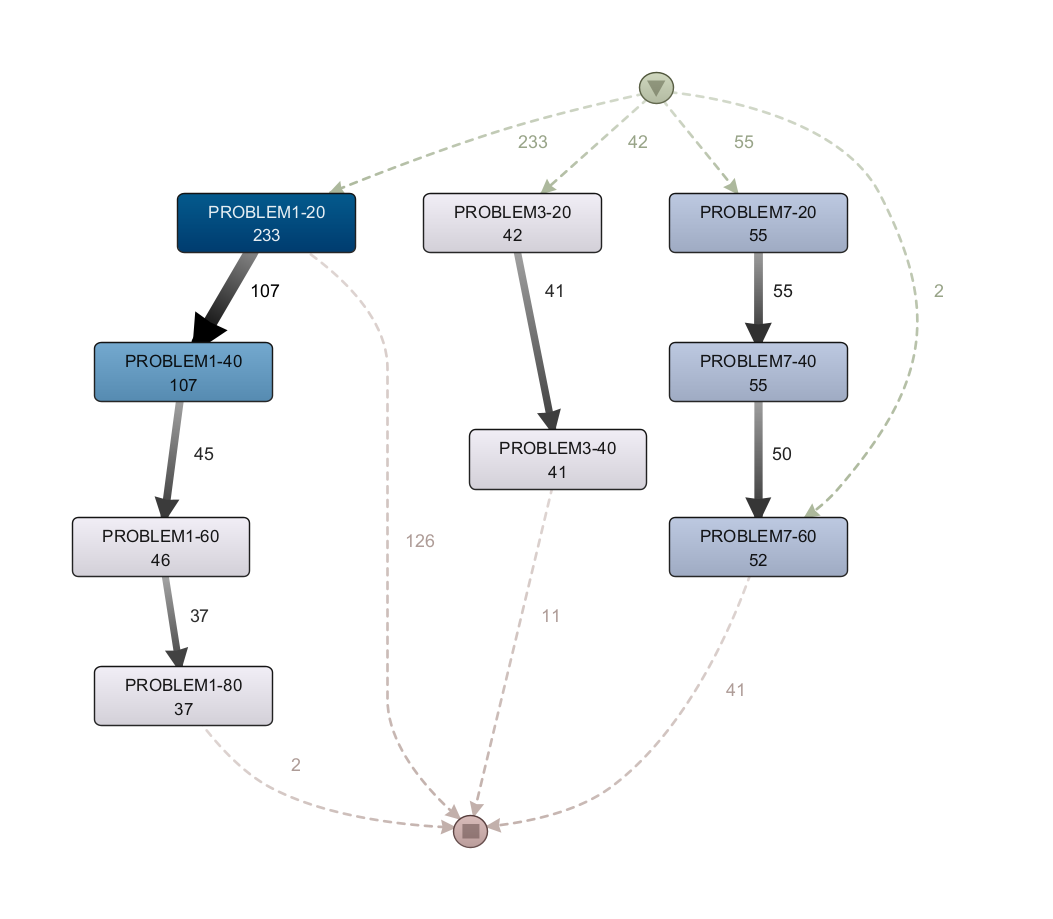
\includegraphics[width=1.25\textwidth]{imagenes/DISCO_compound/Year1920WorstGrades.png}
    \caption{Extracción de procesos del dataset integrado por las acciones compuestas de los grupos con calificación \emph{``baja''} del curso académico 1920.}
    \label{fig:year1920WorstGrades}
\end{figure}

\begin{figure}[H]
    \centering
    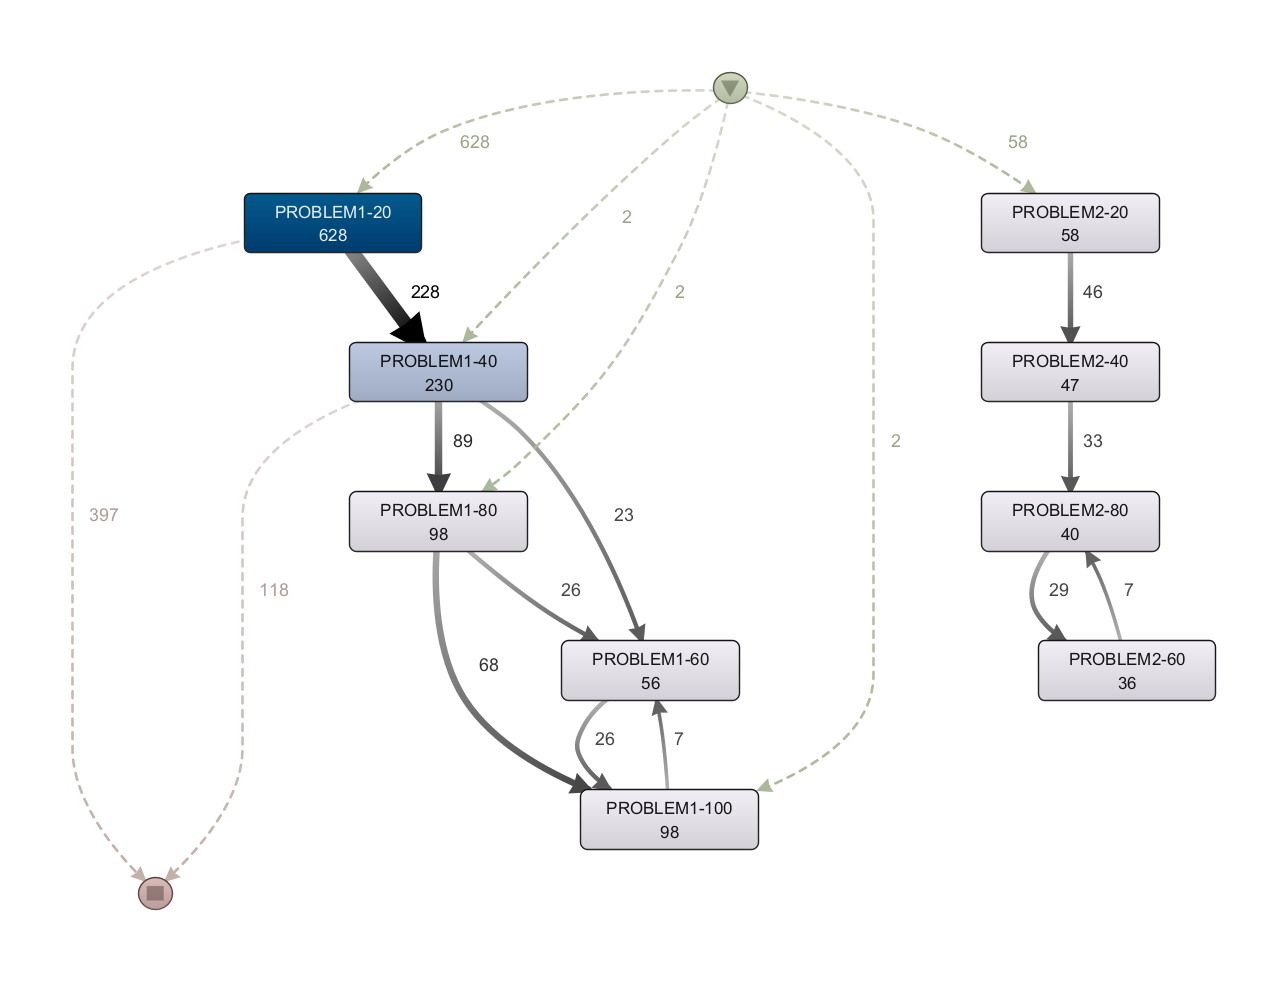
\includegraphics[width=1.25\textwidth]{imagenes/DISCO_compound/Year1516MidLowGrades.png}
    \caption{Extracción de procesos del dataset integrado por las acciones compuestas de los grupos con calificación \emph{``media-baja''} del curso académico 1516.}
    \label{fig:year1516MidLowGrades}
\end{figure}

\begin{figure}[H]
    \centering
    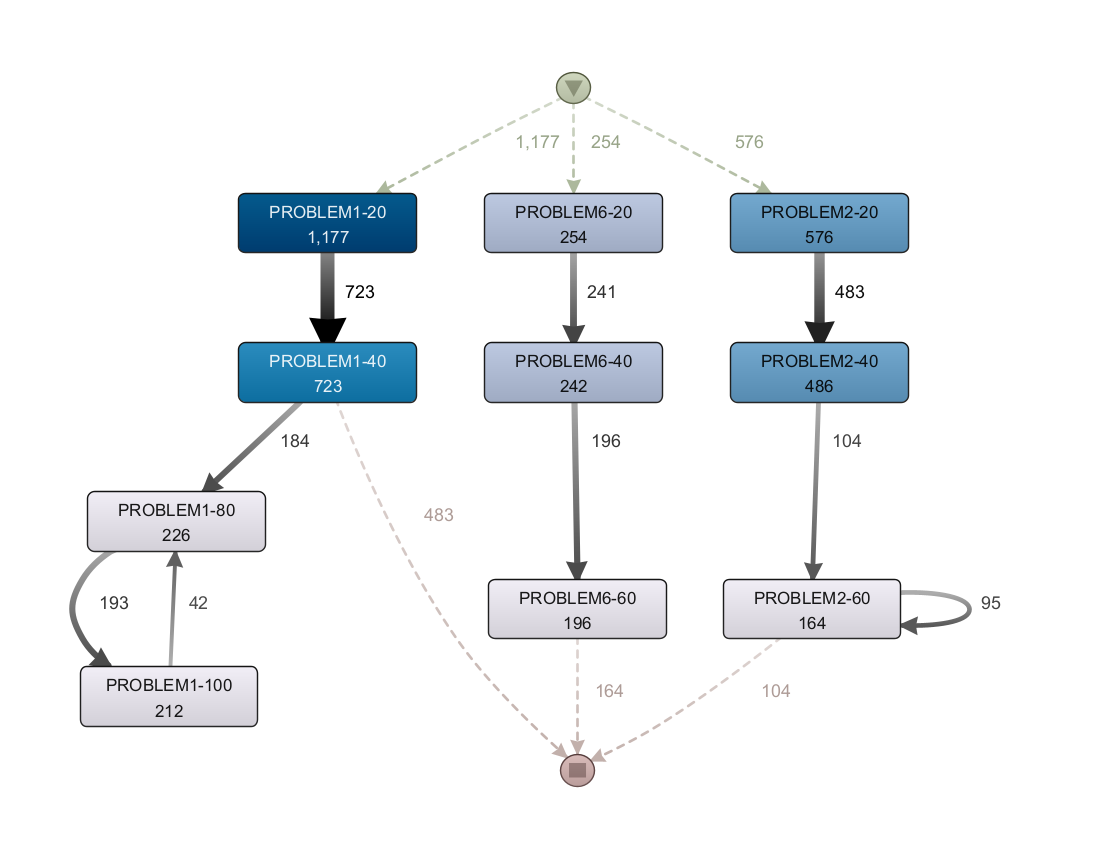
\includegraphics[width=1.25\textwidth]{imagenes/DISCO_compound/Year1718MidLowGrades.png}
    \caption{Extracción de procesos del dataset integrado por las acciones compuestas de los grupos con calificación \emph{``media-baja''} del curso académico 1718.}
    \label{fig:year1718MidLowGrades}
\end{figure}

\begin{figure}[H]
    \centering
    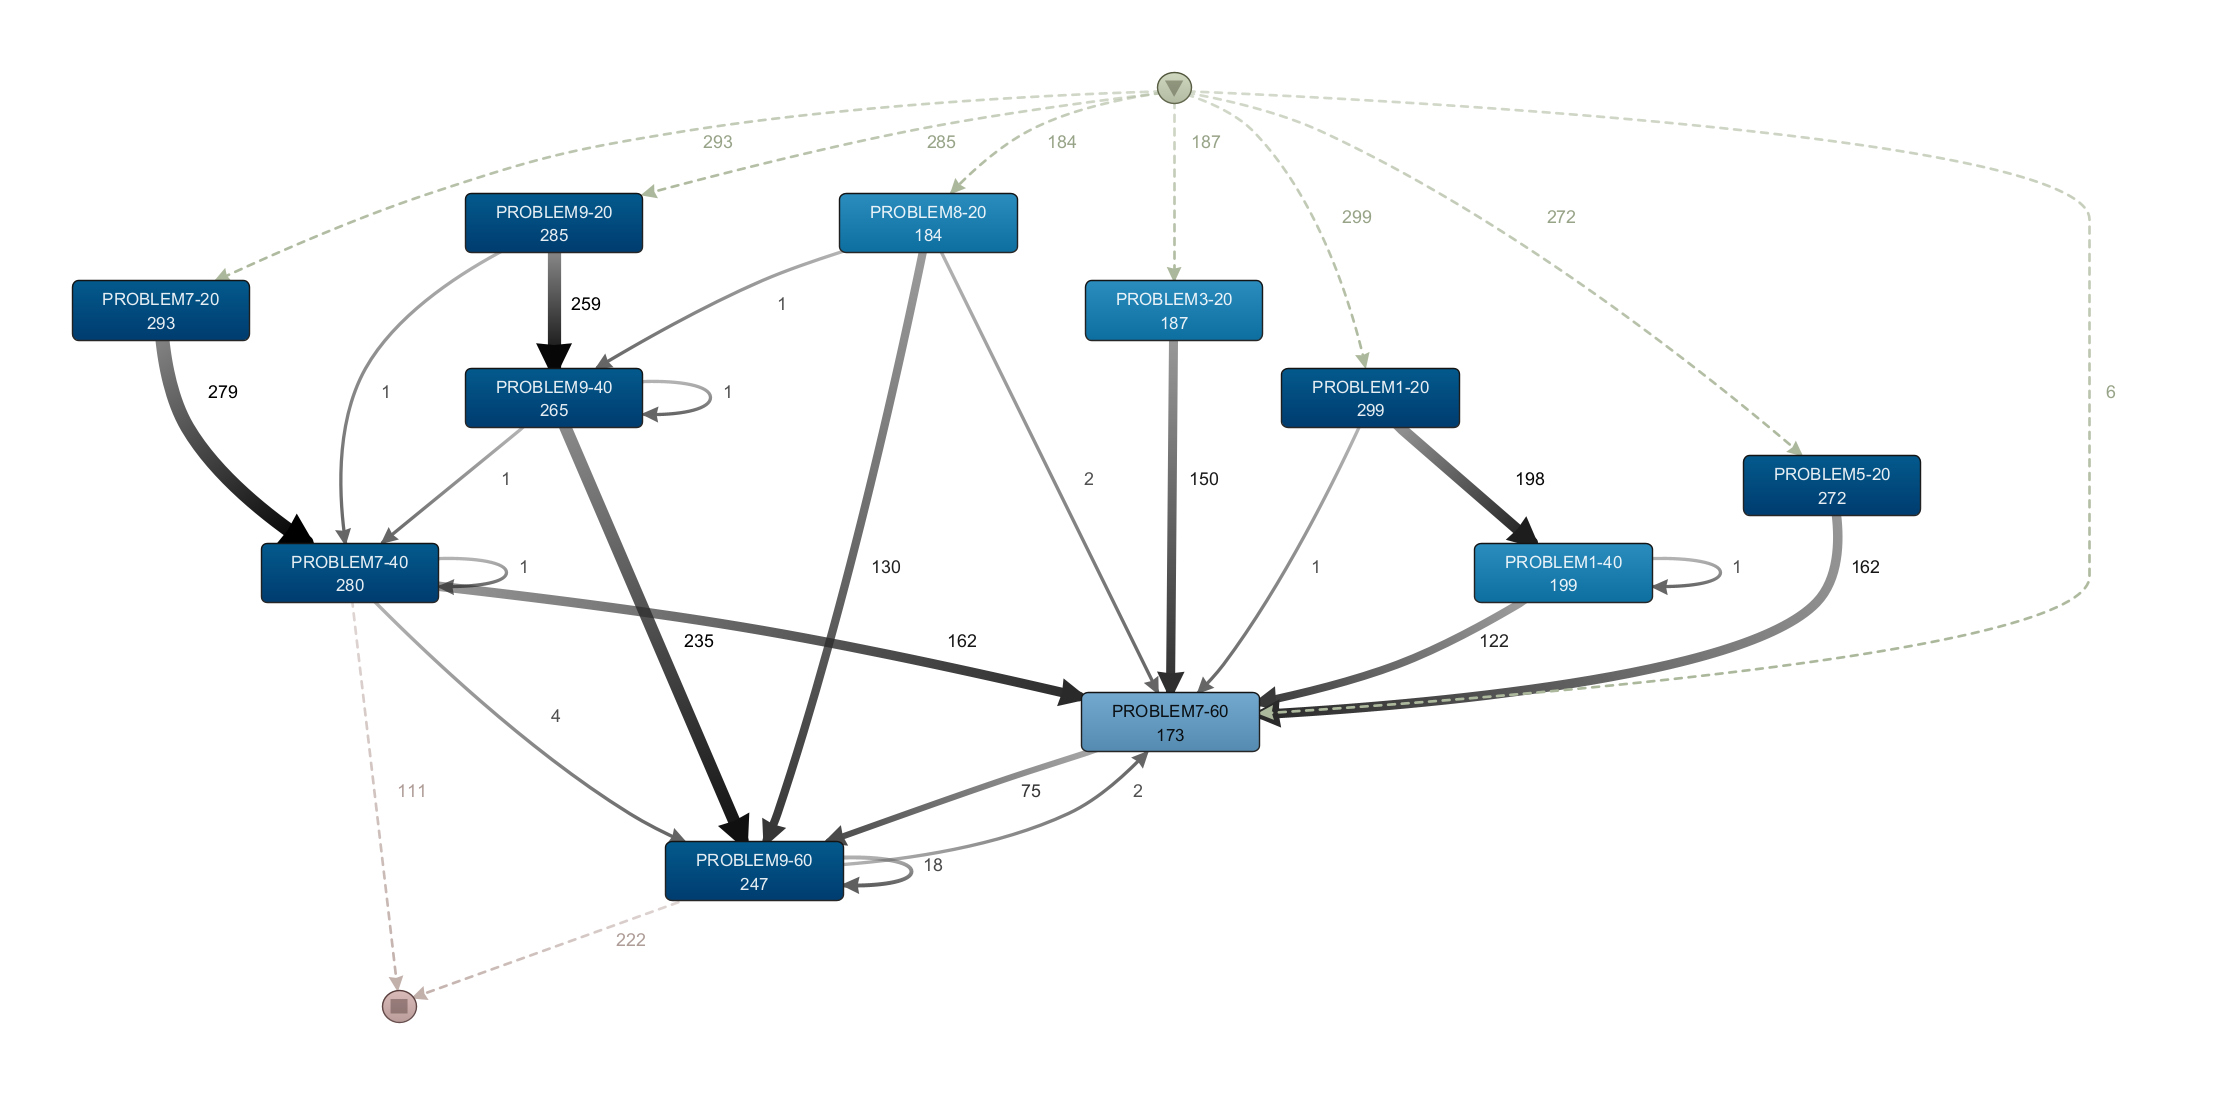
\includegraphics[width=1.25\textwidth]{imagenes/DISCO_compound/Year1920MidLowGrades.png}
    \caption{Extracción de procesos del dataset integrado por las acciones compuestas de los grupos con calificación \emph{``media-baja''} del curso académico 1920.}
    \label{fig:year1920MidLowGrades}
\end{figure}

\begin{figure}[H]
    \centering
    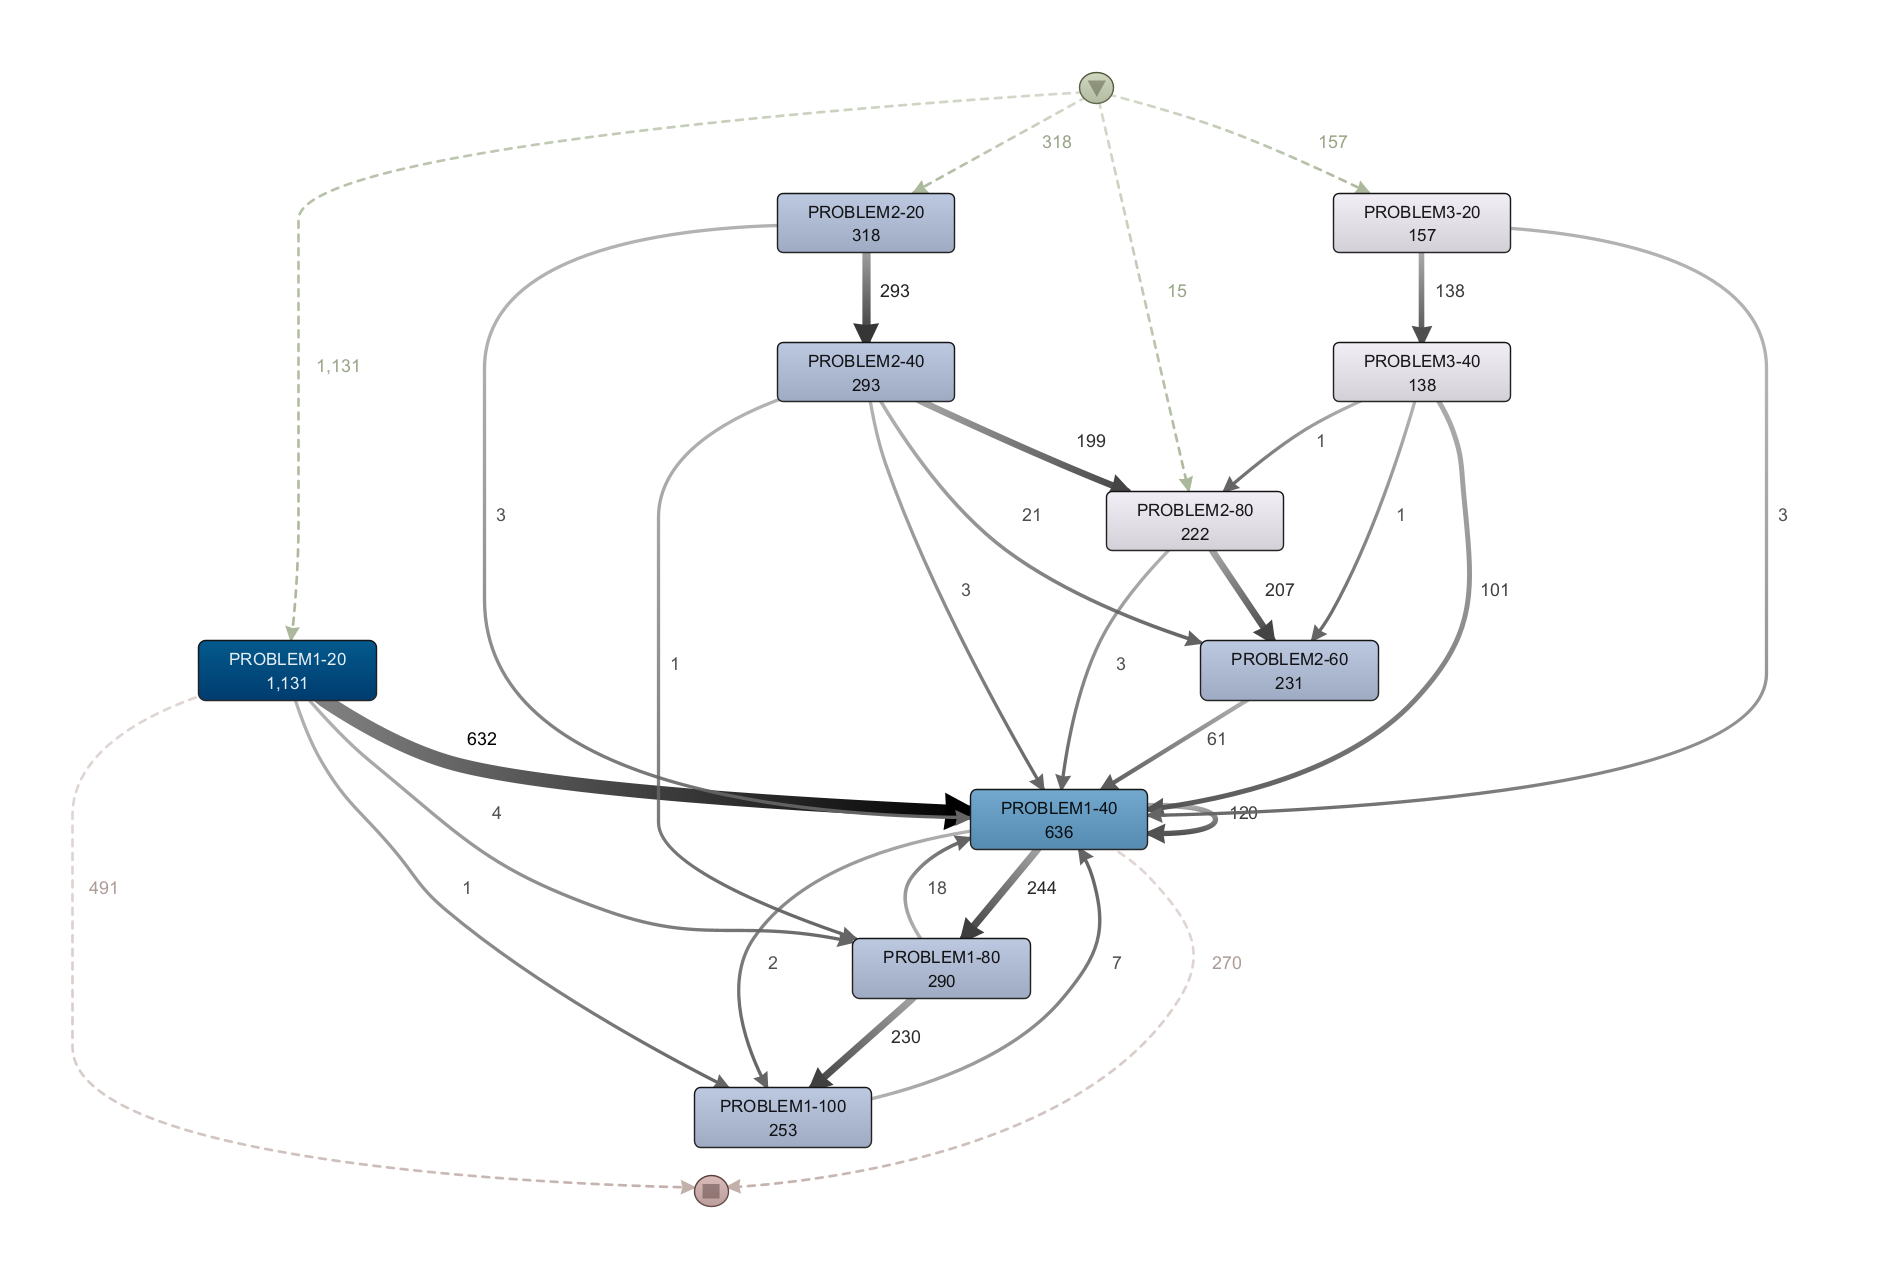
\includegraphics[width=1.25\textwidth]{imagenes/DISCO_compound/Year1516MidHighGrades.png}
    \caption{Extracción de procesos del dataset integrado por las acciones compuestas de los grupos con calificación \emph{``media-alta''} del curso académico 1516.}
    \label{fig:year1516MidHighGrades}
\end{figure}

\begin{figure}[H]
    \centering
    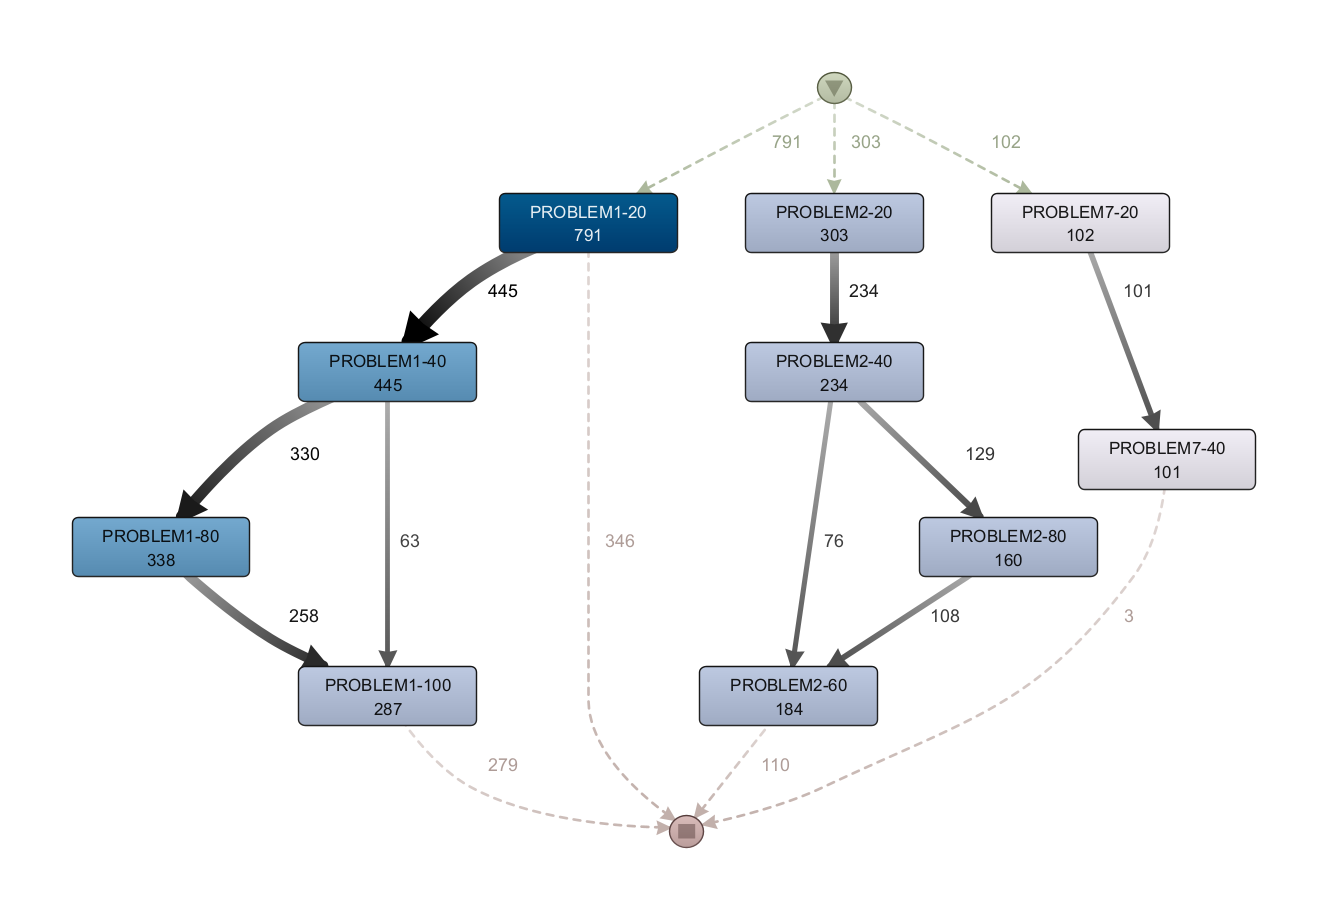
\includegraphics[width=1.25\textwidth]{imagenes/DISCO_compound/Year1617MidHighGrades.png}
    \caption{Extracción de procesos del dataset integrado por las acciones compuestas de los grupos con calificación \emph{``media-alta''} del curso académico 1617.}
    \label{fig:year1617MidHighGrades}
\end{figure}

\begin{figure}[H]
    \centering
    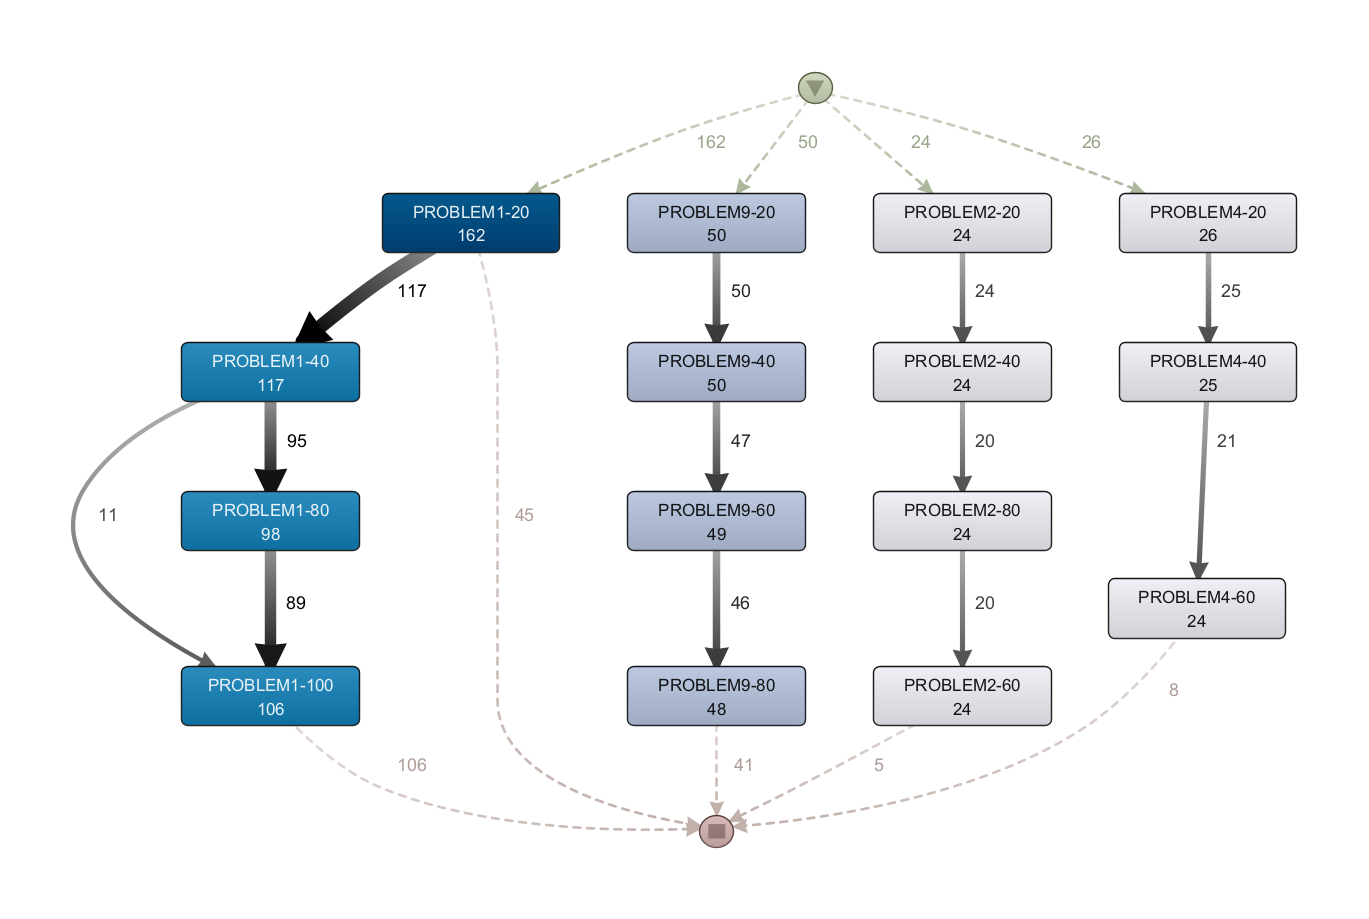
\includegraphics[width=1.25\textwidth]{imagenes/DISCO_compound/Year1718MidHighGrades.png}
    \caption{Extracción de procesos del dataset integrado por las acciones compuestas de los grupos con calificación \emph{``media-alta''} del curso académico 1718.}
    \label{fig:year1718MidHighGrades}
\end{figure}

\begin{figure}[H]
    \centering
    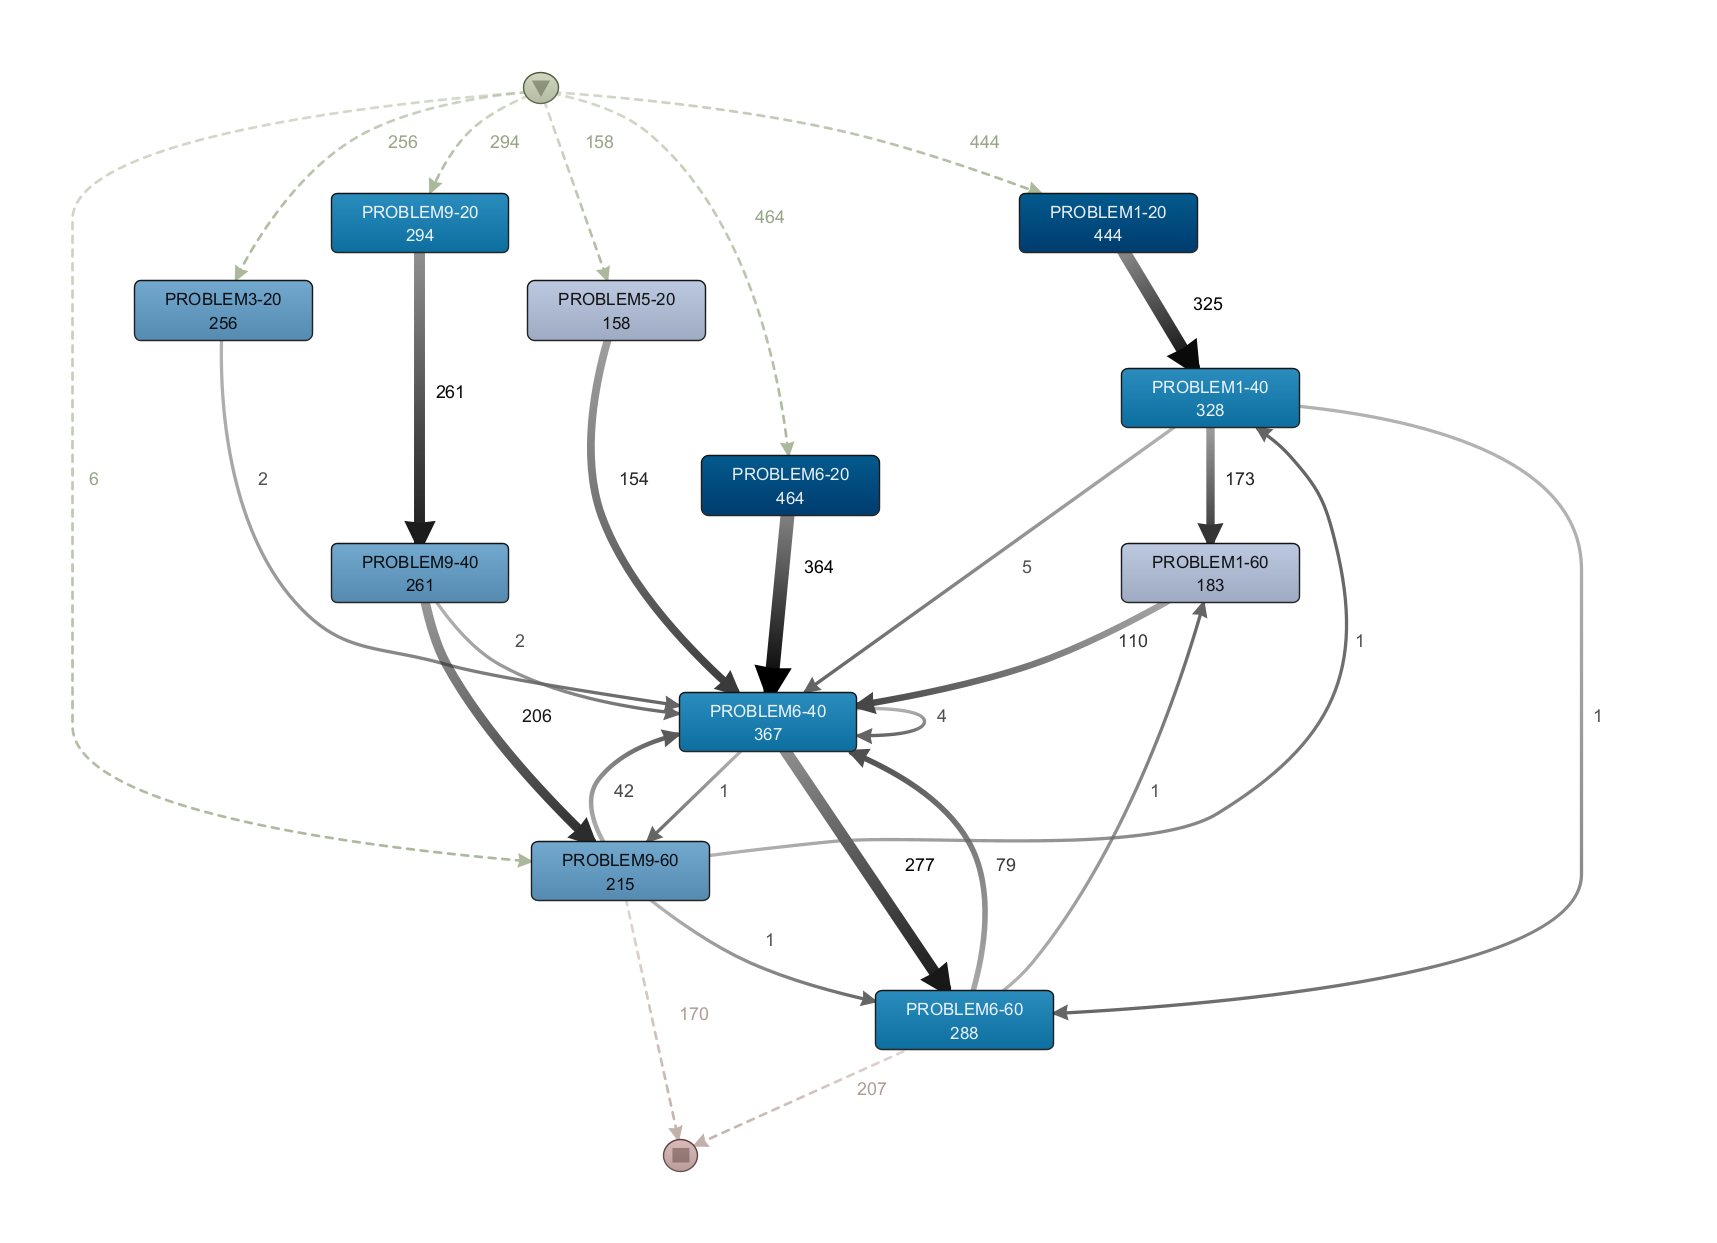
\includegraphics[width=1.25\textwidth]{imagenes/DISCO_compound/Year1920MidHighGrades.png}
    \caption{Extracción de procesos del dataset integrado por las acciones compuestas de los grupos con calificación \emph{``media-alta''} del curso académico 1920.}
    \label{fig:year1920MidHighGrades}
\end{figure}

\begin{figure}[H]
    \centering
    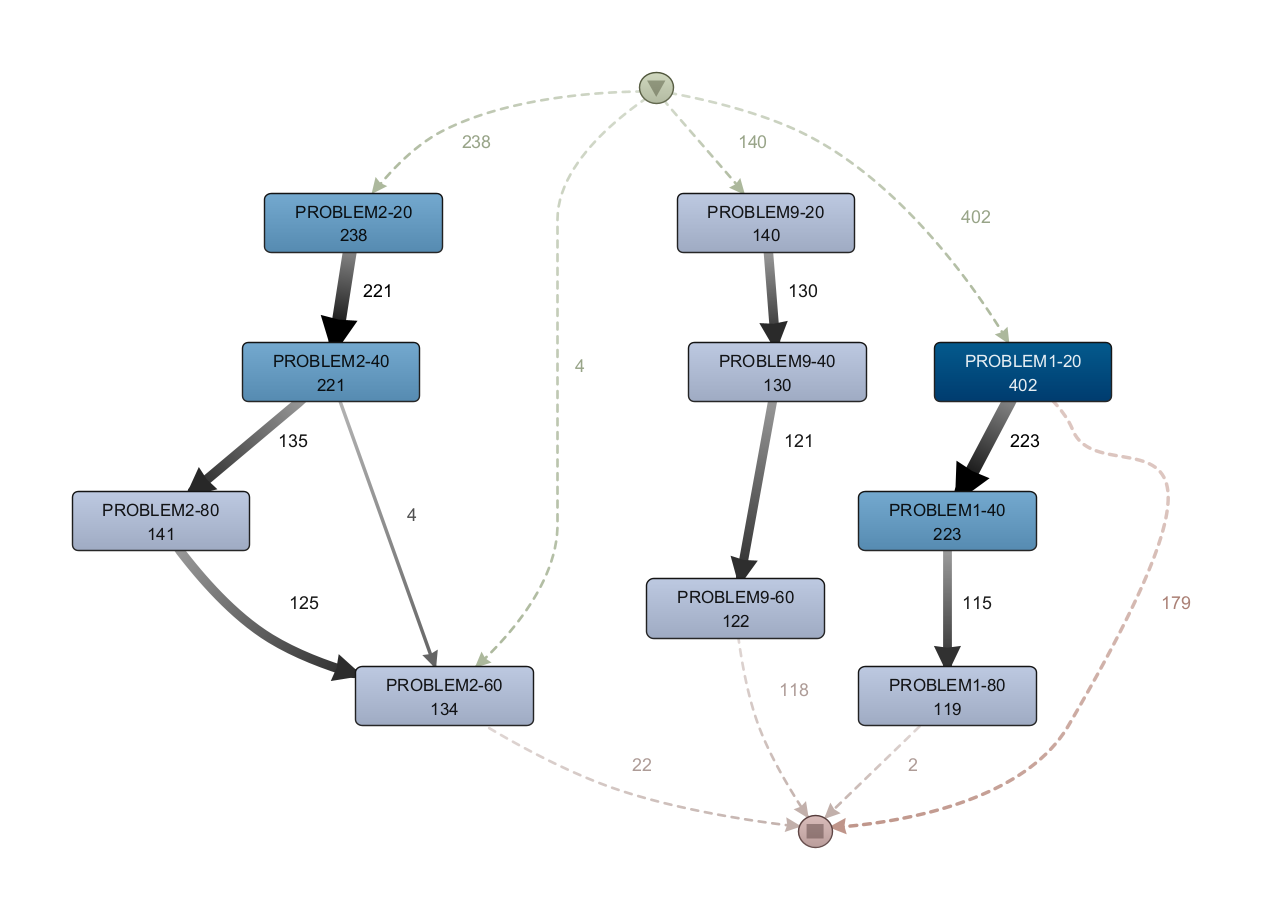
\includegraphics[width=1.25\textwidth]{imagenes/DISCO_compound/Year1516HighGrades.png}
    \caption{Extracción de procesos del dataset integrado por las acciones compuestas de los grupos con calificación \emph{``alta''} del curso académico 1516.}
    \label{fig:year1516BestGrades}
\end{figure}

\begin{figure}[H]
    \centering
    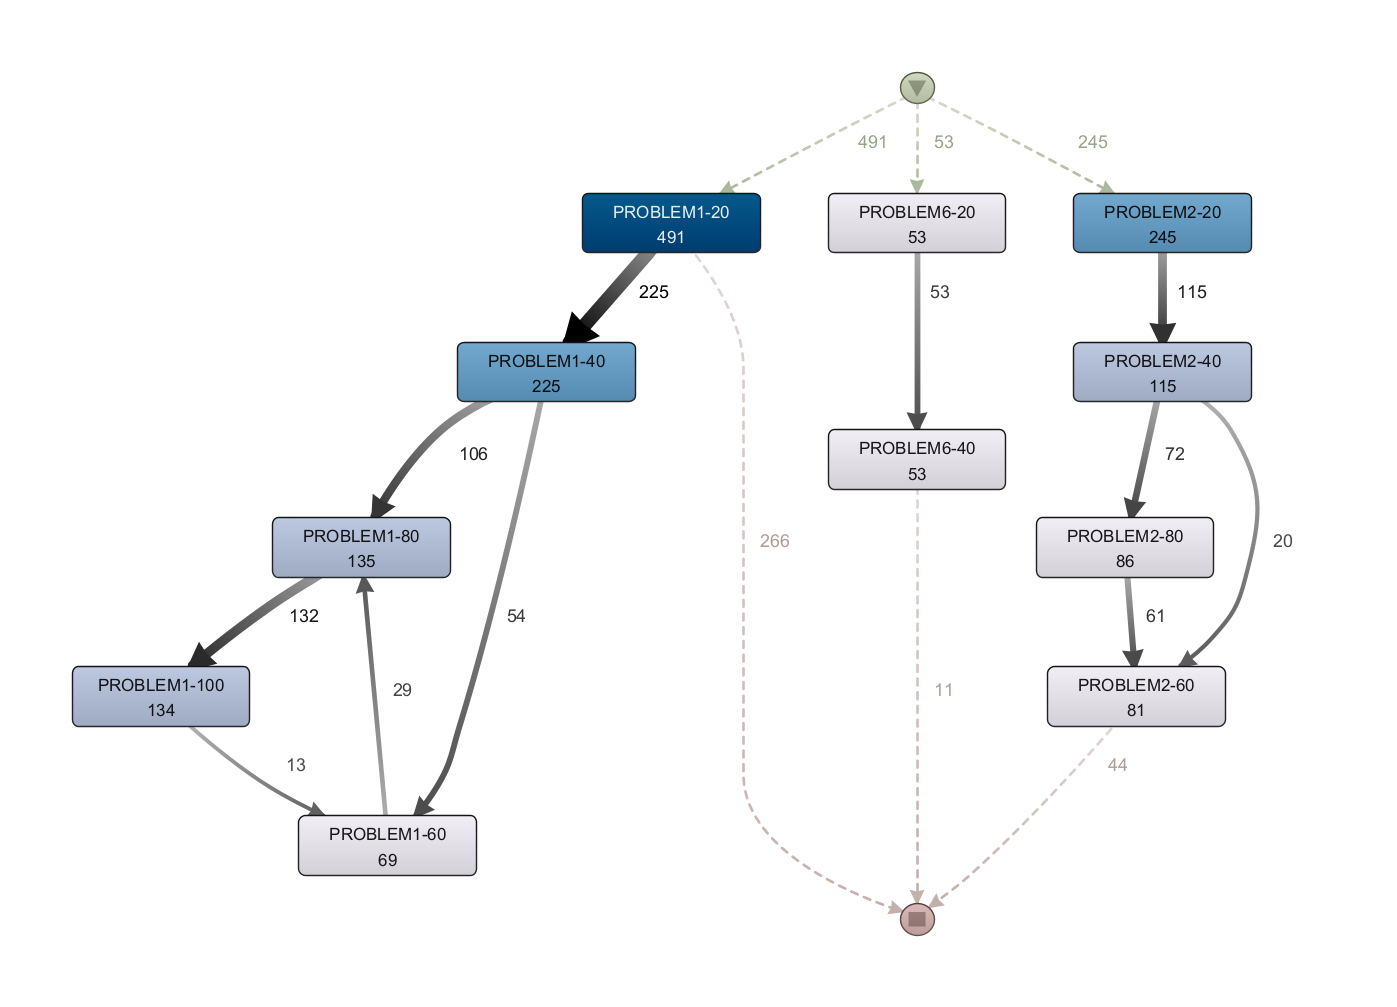
\includegraphics[width=1.25\textwidth]{imagenes/DISCO_compound/Year1617HighGrades.png}
    \caption{Extracción de procesos del dataset integrado por las acciones compuestas de los grupos con calificación \emph{``alta''} del curso académico 1617.}
    \label{fig:year1617BestGrades}
\end{figure}

\begin{figure}[H]
    \centering
    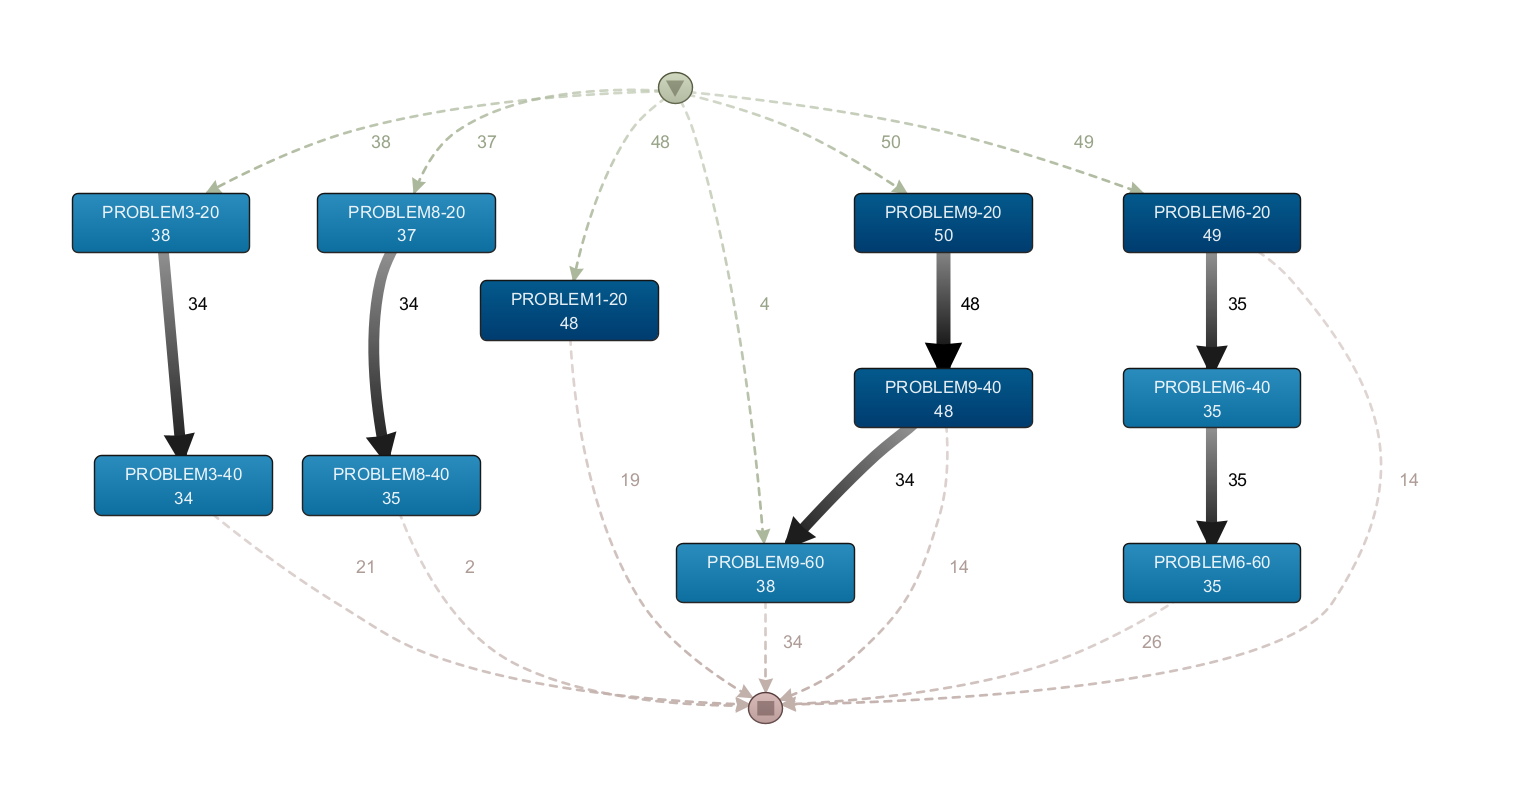
\includegraphics[width=1.25\textwidth]{imagenes/DISCO_compound/Year1920HighGrades.png}
    \caption{Extracción de procesos del dataset integrado por las acciones compuestas de los grupos con calificación \emph{``alta''} del curso académico 1920.}
    \label{fig:year1920BestGrades}
\end{figure}

Como podemos ver en las Figuras \ref{fig:year1516BestGrades}, \ref{fig:year1617BestGrades} y \ref{fig:year1920BestGrades}, el problema $2$ cobra importancia así como otros terceros problemas que varían en función del año:
\begin{itemize}
\item El problema $9$ es el tercero más frecuentado en el curso 1516.
\item El problema $6$ ocupa el tercer puesto en el año académico 1617.
\item El año 1920 presenta diferencias. El nodo más visitado es el \texttt{PROBLEM9-20} (frecuencia $50$), seguido de los nodos \texttt{PROBLEM6-20}, \texttt{PROBLEM1-20}, \texttt{PROBLEM3-20} y \texttt{PROBLEM3-20} (con frecuencias $49$, $48$, $38$ y $37$ respectivamente).
\end{itemize}

Por último, cabe descatar que parece que hay una tendencia a resolver los problemas de manera más secuencial en los procesos extraídos con los grupos de calificaciones más altas. Esto puede observarse claramente si se siguen todas las Figuras de este apartado correspondientes al curso académico 1920 (Figuras \ref{fig:year1920WorstGrades}, \ref{fig:year1920MidLowGrades}, \ref{fig:year1920MidHighGrades} y \ref{fig:year1920BestGrades}).